\documentclass[12pt, a4paper]{article}

% ==========================================
% 1. KHAI BÁO GÓI THƯ VIỆN (PACKAGES)
% ==========================================
% Bảng mã & Font chữ
\usepackage[utf8]{inputenc}
\usepackage[T5]{fontenc}

% Toán học
\usepackage{amsmath, amssymb}

% Căn lề & Bố cục trang
\usepackage[top=2.2cm, bottom=1.5cm, left=1cm, right=1cm, headheight=15pt]{geometry}
\usepackage{fancyhdr}
\usepackage{needspace}
\usepackage{tkz-tab}

% Đồ họa & Màu sắc
\usepackage{xcolor}
\usepackage{graphicx} 
\usepackage{tikz}
\usetikzlibrary{calc, shapes.geometric, positioning}


% Bảng biểu & Danh sách
\usepackage{colortbl}
\usepackage{array}
\usepackage{makecell}
\usepackage{multirow}
\usepackage{tasks}

% Biểu tượng
\usepackage{fontawesome5}

% ==========================================
% 2. THIẾT LẬP MÀU SẮC CHỦ ĐẠO
% ==========================================
\definecolor{goldyellow}{RGB}{255, 179, 0}
\definecolor{amberorange}{RGB}{230, 115, 0}
\definecolor{lightamber}{RGB}{255, 248, 225}
\definecolor{deepblue}{RGB}{25, 42, 86}
\definecolor{accentred}{RGB}{232, 65, 24}
\definecolor{softgray}{RGB}{220, 220, 222} 
\definecolor{fbblue}{RGB}{15, 80, 200}


% ==========================================
% 3. CẤU HÌNH HEADER & FOOTER
% ==========================================
\pagestyle{fancy}
\fancyhf{}
\renewcommand{\headrulewidth}{0pt}

% Khai báo biến lưu trữ nội dung góc phải của Header
\newcommand{\HeaderRightText}{}

% --- Header ---
\fancyhead[C]{
    \begin{tikzpicture}[remember picture, overlay]
        
        % Dải màu trang trí góc trên
        \path[fill=deepblue] (current page.north west) -- (current page.north east) 
            -- ($(current page.north east) + (0, -1.6cm)$) 
            .. controls ($(current page.north) + (3, -2.0cm)$) and ($(current page.north) + (-3, -0.4cm)$) .. 
            ($(current page.north west) + (0, -1.0cm)$) -- cycle;
            
        \path[fill=goldyellow] (current page.north west) -- (current page.north east) 
            -- ($(current page.north east) + (0, -1.0cm)$) 
            .. controls ($(current page.north) + (4, -1.0cm)$) and ($(current page.north) + (-2, -2.2cm)$) .. 
            ($(current page.north west) + (0, -1.6cm)$) -- cycle;
            
        \path[fill=amberorange] (current page.north west) -- ($(current page.north west) + (6.5cm, 0)$) 
            .. controls ($(current page.north west) + (4.5cm, -1.2cm)$) and ($(current page.north west) + (2cm, -2.0cm)$) .. 
            ($(current page.north west) + (0, -2.0cm)$) -- cycle;
            
        % Logo góc trái Header
        \node[anchor=west, inner sep=0pt] 
            at ($(current page.north west) + (0cm, -0.8cm)$) {
\includegraphics[height=2.0cm]{../../../image/logo-header.png}};
            
        % Text góc phải Header (Tự động lấy từ đối số thứ 3 của \titlebox)
        \node[anchor=east, text=white, font=\small\bfseries\sffamily] 
            at ($(current page.north east) + (-0.8cm, -0.5cm)$) {\HeaderRightText};
    \end{tikzpicture}
}

% --- Footer ---
\fancyfoot[C]{
    \begin{tikzpicture}[remember picture, overlay]
        % Đường kẻ ngang
        \draw[amberorange, line width=1.5pt] 
            ($(current page.south west) + (0cm, 0.4cm)$) -- ($(current page.south east) + (0cm, 0.4cm)$);

        % Dải cong góc phải
        \path[fill=goldyellow] (current page.south east) -- ($(current page.south east) + (-5cm, 0)$) 
            .. controls ($(current page.south east) + (-3cm, 0.8cm)$) and ($(current page.south east) + (-1.5cm, 1.2cm)$) .. 
            ($(current page.south east) + (0, 1.2cm)$) -- cycle;

        % Mạng xã hội
        \node[anchor=west, inner sep=0pt] at ($(current page.south west) + (1cm, 0.8cm)$) {
            \small\sffamily
            \textcolor{fbblue}{\faFacebook\hskip 4pt Toán Anh Huy MATH-STER}
            \hskip 18pt
            \textcolor{black}{\faTiktok\hskip 4pt huymathster}
        };

        % Số trang
        \node[circle, fill=white, draw=amberorange, line width=1.5pt, text=deepblue, font=\large\bfseries\sffamily, inner sep=4pt, minimum size=0.8cm] 
            at ($(current page.south east) + (-1.2cm, 0.6cm)$) {\thepage};
    \end{tikzpicture}
}

% ==========================================
% 4. ĐỊNH NGHĨA MACRO: KHUNG TIÊU ĐỀ
% ==========================================
\newcommand{\titlebox}[3]{
    % Gán nội dung đối số #3 vào biến HeaderRightText
    \gdef\HeaderRightText{#3}
    
    \begin{center}
    \vspace*{-0.5cm}
    \begin{tikzpicture}
        % Khung vô hình (Phantom Box) định chuẩn kích thước
        \node[text width=16cm, inner xsep=0pt, inner ysep=16pt, opacity=0] (MainBox) {
            \begin{minipage}[c]{4.2cm}
                \centering\vspace{0.1cm}
                \rule{2.2cm}{2.2cm} 
                \vspace{0.1cm}
            \end{minipage}%
            \begin{minipage}[c]{11.5cm}
                \centering\vspace{0.15cm}
                {\huge\bfseries\sffamily #2 \par}
                \vspace{0.15cm} 
            \end{minipage}
        };
        
        % Đổ bóng & Nền
        \fill[goldyellow, rounded corners=8pt] ([xshift=5pt, yshift=-5pt]MainBox.south west) rectangle ([xshift=5pt, yshift=-5pt]MainBox.north east);
        \fill[white, rounded corners=8pt] (MainBox.south west) rectangle (MainBox.north east);
        
        % Lưới ô ly & Nền Logo
        \begin{scope}
            \clip[rounded corners=8pt] (MainBox.south west) rectangle (MainBox.north east);
            \draw[step=0.4cm, softgray!50, line width=0.6pt] (MainBox.south west) grid (MainBox.north east);
            \fill[lightamber!60] (MainBox.south west) rectangle ([xshift=4.2cm]MainBox.north west);
        \end{scope}

        % Viền ngoài
        \draw[deepblue, line width=1.5pt, rounded corners=8pt] (MainBox.south west) rectangle (MainBox.north east);

        % Nội dung Text (Lớp trên cùng)
        \node[text width=16cm, inner xsep=0pt, inner ysep=16pt] at (MainBox.center) {
            \begin{minipage}[c]{4.2cm}
                \centering
                % --- ĐIỀU CHỈNH TỌA ĐỘ LOGO Ở ĐÂY ---
                \hspace*{-0.5cm}\raisebox{-0.2cm}{
\includegraphics[width=5.5cm]{../../../image/logo.png}}
            \end{minipage}%
            \begin{minipage}[c]{11.5cm}
                \centering\vspace{0.15cm}
                {\huge\bfseries\sffamily\color{deepblue} #2 \par}
                \vspace{0.15cm} 
            \end{minipage}
        };
        
        % Trang trí phụ kiện
        \draw[deepblue, line width=1.5pt, dashed] ([xshift=4.2cm]MainBox.north west) -- ([xshift=4.2cm]MainBox.south west);
        \node[regular polygon, regular polygon sides=4, rotate=45, fill=white, draw=accentred, line width=1.2pt, inner sep=2.5pt] at ([xshift=4.2cm]MainBox.west) {};
        \node[anchor=west, fill=amberorange, text=white, font=\large\bfseries\sffamily, rounded corners=4pt, draw=deepblue, line width=1.5pt, inner xsep=12pt, inner ysep=6pt] at ([xshift=1.5cm]MainBox.north west) {#1};
        \fill[accentred] ([xshift=-1.8cm, yshift=-0.4cm]MainBox.north east) circle (3pt);
        \fill[amberorange] ([xshift=-1.4cm, yshift=-0.4cm]MainBox.north east) circle (3pt);
        \fill[goldyellow] ([xshift=-1.0cm, yshift=-0.4cm]MainBox.north east) circle (3pt);
    \end{tikzpicture}
    \vspace*{0cm}
    \end{center}
}

% ==========================================
% 5. ĐỊNH NGHĨA MACRO: CẤU TRÚC CÂU HỎI (ÉP SÁT NHAU)
% ==========================================
\newcommand{\questioncore}[2]{
    % Xóa khoảng cách phía trên, ép sát câu trước
    \noindent \textbf{\textcolor{deepblue}{Câu #1.} \textcolor{accentred}{[STER]}} #2
    \par\nopagebreak
}

% Cấu hình hiển thị đáp án trắc nghiệm
\settasks{
    label=\textbf{\textcolor{amberorange}{\Alph*.}}, 
    label-width=15pt,     
    item-indent=25pt,     
    label-offset=6pt,    
    column-sep=20pt,     
    after-item-skip=2pt  % Đã giảm tối đa khoảng cách giữa các dòng đáp án A B C D
}

% Hàm vẽ dòng kẻ nháp
\newcommand{\drawdashlines}[1]{
    \ifnum#1>0
        \nopagebreak\vspace{0.1cm}\noindent 
        \begin{tikzpicture}
            \foreach \i in {1,...,#1} {
                \draw[softgray, line width=0.2pt] (0,-{\i*0.65}) -- (\textwidth-4pt,-{\i*0.65});
            }
        \end{tikzpicture}
        \par
    \fi
    % Đã xóa hoàn toàn khoảng cách thừa ở nhánh else
}

% --- Dạng 1: Trắc nghiệm 4 đáp án ---
\newcommand{\questionLinesManual}[4]{
    \pgfmathsetmacro{\calculatedSpace}{1.5 + #1 * 0.65}
    \needspace{\calculatedSpace cm} 
    \questioncore{#2}{#3}
    #4
    \par\nopagebreak
    \drawdashlines{#1}
}

% --- Dạng 2: Trắc nghiệm Đúng/Sai ---
\newcommand{\questionTrueFalse}[4]{
    \pgfmathsetmacro{\calculatedSpace}{3.0 + #1 * 0.65} 
    \needspace{\calculatedSpace cm}
    \questioncore{#2}{#3}
    
    \nopagebreak
    \begin{center}
    \renewcommand{\arraystretch}{1.2} % Bóp nhỏ chiều cao của bảng Đ/S
    \begin{tabular}{|>{\centering\arraybackslash}m{0.8cm}|m{12cm}|>{\centering\arraybackslash}m{2cm}|>{\centering\arraybackslash}m{2cm}|}
        \hline
        \rowcolor{amberorange!20}
        & \multicolumn{1}{>{\centering\arraybackslash}m{12cm}|}{\textbf{\textcolor{deepblue}{Mệnh đề}}} & 
        \textbf{\textcolor{deepblue}{Đúng}} & 
        \textbf{\textcolor{deepblue}{Sai}} \\
        \hline
        #4
        \hline
    \end{tabular}
    \renewcommand{\arraystretch}{1}
    \end{center}
    
    \par\nopagebreak
    \drawdashlines{#1}
}

% ----- Dạng 3: Tự luận ngắn -----
\newcommand{\questionShortAnswer}[3]{
    \pgfmathsetmacro{\calculatedSpace}{1.5 + #1 * 0.8}
    \needspace{\calculatedSpace cm}
    
    {\linespread{1.1}\selectfont % Bóp nhỏ giãn dòng của câu tự luận
    \questioncore{#2}{#3}\par}
    
    \nopagebreak
    \begin{flushright}
        \begin{tikzpicture}
            \node[anchor=east, font=\small\bfseries\sffamily, text=deepblue] 
                at (-0.2, 0.4) {Đáp án:};
            \fill[goldyellow, rounded corners=3pt] (0.08, -0.08) rectangle (3.08, 0.72);
            \draw[draw=deepblue, fill=white, line width=1.2pt, rounded corners=3pt] 
                (0,0) rectangle (3.0, 0.8);
            \foreach \x in {0.75, 1.5, 2.25} {
                \draw[draw=deepblue, line width=0.6pt] (\x, 0) -- (\x, 0.8);
            }
        \end{tikzpicture}
    \end{flushright}
    
    \par\nopagebreak
    \drawdashlines{#1}
}

% ==========================================
% BẮT ĐẦU NỘI DUNG TÀI LIỆU
% ==========================================
\begin{document}

% Truyền 3 tham số: {Nhãn cam} {Chữ to chính giữa} {Chữ ở góc phải Header}
\titlebox{Chủ đề: Hàm số}{Khảo sát hàm số bậc 3}{Hàm số: Hàm bậc 3}

% --- CÂU 1 ---
\questionLinesManual{0}{1}{Đồ thị của hàm số nào dưới đây có dạng như đường cong trong hình bên?

\begin{center}
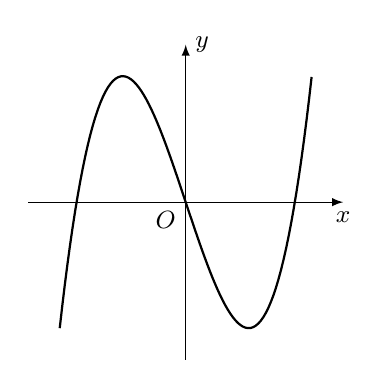
\begin{tikzpicture}[>=latex, scale=0.8]
    % Hệ trục tọa độ
    \draw[->] (-2.5,0) -- (2.5,0) node[below] {\small $x$};
    \draw[->] (0,-2.5) -- (0,2.5) node[right] {\small $y$};
    \node[below left] at (0,0) {\small $O$};
    
    % Đồ thị hàm bậc 3: y = x^3 - 3x
    \draw[thick, samples=100, domain=-2:2] 
        plot (\x, {\x*\x*\x - 3*\x});
    
\end{tikzpicture}
\end{center}

}{
    \begin{tasks}(4)
        \task \( y = x^3 - 3x \)
        \task \( y = -x^3 + 3x \)
        \task \( y = x^4 - 2x^2 \)
        \task \( y = -x^4 + 2x^2 \)
    \end{tasks}
}

% --- CÂU 2 ---
\questionLinesManual{0}{2}{Đồ thị hàm số nào dưới đây có dạng như đường cong hình bên

\begin{center}
\begin{tikzpicture}[>=latex, scale=0.8]
    % Hệ trục tọa độ
    \draw[->] (-2.5,0) -- (2.5,0) node[below] {\small $x$};
    \draw[->] (0,-3.5) -- (0,1.5) node[right] {\small $y$};
    \node[below left] at (0,0) {\small $O$};
    
    % Đồ thị hàm bậc 4 trùng phương: y = -x^4 + 2x^2 - 2
    \draw[thick, samples=100, domain=-1:2.3] 
        plot (\x, {-\x*\x*\x+2*\x*\x - 2});
    
\end{tikzpicture}
\end{center}

}{
    \begin{tasks}(4)
        \task \( y = x^4 - 2x^2 - 2 \)
        \task \( y = -x^3 + 2x^2 - 2 \)
        \task \( y = x^3 - 3x^2 - 2 \)
        \task \( y = -x^4 + 2x^2 - 2 \)
    \end{tasks}
}

% --- CÂU 3 ---
\questionLinesManual{0}{3}{Đường cong hình bên là đồ thị của một trong bốn hàm số dưới đây. Hàm số đó là hàm số nào?

\begin{center}
\begin{tikzpicture}[>=latex, scale=0.8]
    % Hệ trục tọa độ
    \draw[->] (-3.5,0) -- (3.5,0) node[below] {\small $x$};
    \draw[->] (0,-2.5) -- (0,5.5) node[right] {\small $y$};
    \node[below left] at (0,0) {\small $O$};
    
    % Đồ thị hàm bậc 3: y = -x^3 + 3x + 2
    \draw[thick, samples=100, domain=-2.2:2.1] 
        plot (\x, {\x*\x*\x - 3*\x + 2});
    
  
\end{tikzpicture}
\end{center}

}{
    \begin{tasks}(4)
        \task \( y = -x^3 + 3x + 2 \)
        \task \( y = x^4 - x^2 + 1 \)
        \task \( y = x^4 + x^2 + 1 \)
        \task \( y = x^3 - 3x + 2 \)
    \end{tasks}
}

% --- CÂU 4 ---
\questionLinesManual{0}{4}{Đồ thị của hàm số nào dưới đây có dạng như đường cong trong hình bên?

\begin{center}
\begin{tikzpicture}[>=latex, scale=0.8]
    % Hệ trục tọa độ
    \draw[->] (-2.5,0) -- (4.5,0) node[below] {\small $x$};
    \draw[->] (0,-2) -- (0,4.5) node[right] {\small $y$};
    \node[above left] at (0,0) {\small $O$};
    
    % Đồ thị hàm bậc 4 trùng phương: y = -x^4 + 2x^2 - 1
    \draw[thick, samples=100, domain=-1.05:3.1] 
        plot (\x, {-\x*\x*\x + 3*\x*\x - 1});
\end{tikzpicture}
\end{center}

}{
    \begin{tasks}(4)
        \task \( y = -x^4 + 2x^2 - 1 \)
        \task \( y = x^4 - 2x^2 - 1 \)
        \task \( y = x^3 - 3x^2 - 1 \)
        \task \( y = -x^3 + 3x^2 - 1 \)
    \end{tasks}
}

% --- CÂU 5 ---
\questionLinesManual{0}{5}{Đồ thị của hàm số dưới đây có dạng như đường cong bên?

\begin{center}
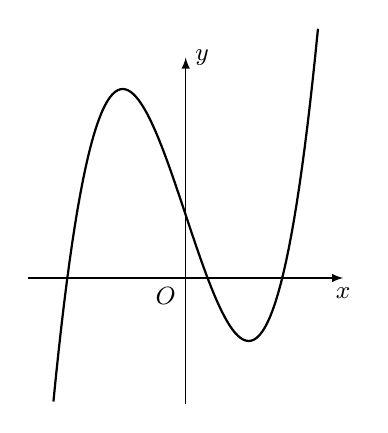
\begin{tikzpicture}[>=latex, scale=0.8]
    % Hệ trục tọa độ
    \draw[->] (-2.5,0) -- (2.5,0) node[below] {\small $x$};
    \draw[->] (0,-2) -- (0,3.5) node[right] {\small $y$};
    \node[below left] at (0,0) {\small $O$};
    
    % Đồ thị hàm bậc 3: y = -x^3 + 3x + 1
    \draw[thick, samples=100, domain=-2.1:2.1] 
        plot (\x, {\x*\x*\x - 3*\x + 1});
\end{tikzpicture}
\end{center}

}{
    \begin{tasks}(4)
        \task \( y = x^3 - 3x + 1 \)
        \task \( y = x^4 - 2x^2 + 1 \)
        \task \( y = -x^4 + 2x^2 + 1 \)
        \task \( y = -x^3 + 3x + 1 \)
    \end{tasks}
}

% --- CÂU 6 ---
\questionLinesManual{0}{6}{Đồ thị của hàm số nào dưới đây có dạng như đường cong trong hình bên?

\begin{center}
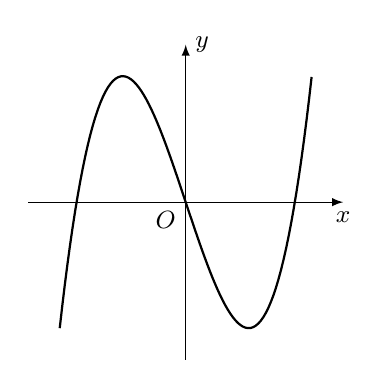
\begin{tikzpicture}[>=latex, scale=0.8]
    % Hệ trục tọa độ
    \draw[->] (-2.5,0) -- (2.5,0) node[below] {\small $x$};
    \draw[->] (0,-2.5) -- (0,2.5) node[right] {\small $y$};
    \node[below left] at (0,0) {\small $O$};
    
    % Đồ thị hàm bậc 3: y = x^3 - 3x
    \draw[thick, samples=100, domain=-2:2] 
        plot (\x, {\x*\x*\x - 3*\x});
\end{tikzpicture}
\end{center}

}{
    \begin{tasks}(4)
        \task \( y = x^4 + 2x^2 \)
        \task \( y = -x^3 - 3x \)
        \task \( y = x^3 - 3x \)
        \task \( y = -x^4 + 2x^2 \)
    \end{tasks}
}

% --- CÂU 7 ---
\questionLinesManual{0}{7}{Đường cong ở hình bên dưới là đồ thị của một trong bốn hàm số dưới đây. Hàm số đó là hàm số nào?

\begin{center}
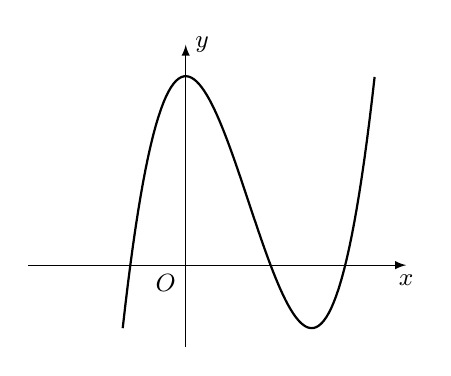
\begin{tikzpicture}[>=latex, scale=0.8]
    % Hệ trục tọa độ
    \draw[->] (-2.5,0) -- (3.5,0) node[below] {\small $x$};
    \draw[->] (0,-1.3) -- (0,3.5) node[right] {\small $y$};
    \node[below left] at (0,0) {\small $O$};
    
    % Đồ thị hàm bậc 4 trùng phương: y = x^4 - 2x^2 + 1
    \draw[thick, samples=100, domain=-1:3] 
        plot (\x, {\x*\x*\x - 3*\x*\x +3});
\end{tikzpicture}
\end{center}

}{
    \begin{tasks}(4)
        \task \( y = -x^3 + 3x^2 + 1 \)
        \task \( y = x^3 - 3x^2 + 3 \)
        \task \( y = -x^4 + 2x^2 + 1 \)
        \task \( y = x^4 - 2x^2 + 1 \)
    \end{tasks}
}

% --- CÂU 8 ---
\questionLinesManual{0}{8}{Đường cong trong hình bên là đồ thị của một hàm số trong bốn hàm số được liệt kê ở bốn phương án dưới đây. Hỏi hàm số đó là hàm số nào?

\begin{center}
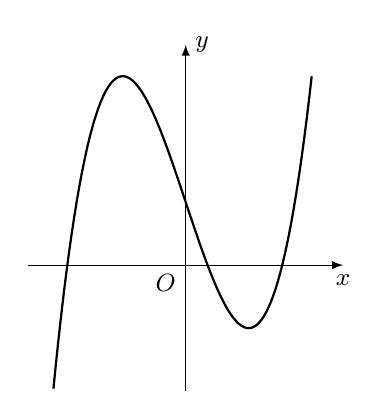
\begin{tikzpicture}[>=latex, scale=0.8]
    % Hệ trục tọa độ
    \draw[->] (-2.5,0) -- (2.5,0) node[below] {\small $x$};
    \draw[->] (0,-2) -- (0,3.5) node[right] {\small $y$};
    \node[below left] at (0,0) {\small $O$};
    
    % Đồ thị hàm bậc 3: y = -x^3 + 3x + 1
    \draw[thick, samples=100, domain=-2.1:2] 
        plot (\x, {\x*\x*\x - 3*\x + 1});
    
\end{tikzpicture}
\end{center}

}{
    \begin{tasks}(4)
        \task \( y = x^3 - 3x + 1 \)
        \task \( y = -x^3 + 3x + 1 \)
        \task \( y = x^4 - x^2 + 1 \)
        \task \( y = -x^2 + x - 1 \)
    \end{tasks}
}

% --- CÂU 9 ---
\questionLinesManual{0}{9}{Đường cong bên là đồ thị hàm số nào sau đây?

\begin{center}
\begin{tikzpicture}[>=latex, scale=0.8]
    % 2. Vẽ hệ trục tọa độ
    \draw[->] (-3.5,0) -- (3.5,0) node[below] {\small $x$};
    \draw[->] (0,-3) -- (0,3.5) node[right] {\small $y$};
    \node[below left] at (0,0) {\small $O$};
    
    % 3. Vẽ đồ thị hàm số y = x^3 - 3x
    \draw[thick, samples=100, domain=-2.1:2.1] 
        plot (\x, {\x*\x*\x - 3*\x});
\end{tikzpicture}
\end{center}

}{
    \begin{tasks}(4)
        \task \( y = x^3 - 3x + 1 \)
        \task \( y = x^3 - 3x \)
        \task \( y = x^3 - 3x - 1 \)
        \task \( y = x^3 + 3x \)
    \end{tasks}
}
% --- CÂU 10 ---
\questionLinesManual{0}{10}{Đồ thị của hàm số nào dưới đây có dạng như đường cong trong hình vẽ bên.

\begin{center}
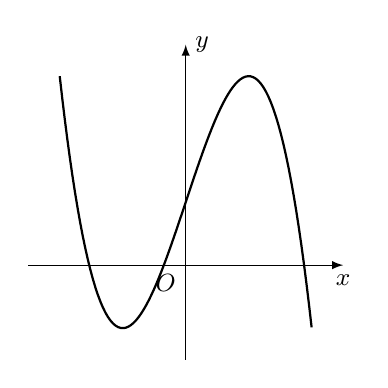
\begin{tikzpicture}[>=latex, scale=0.8]
    % Hệ trục tọa độ
    \draw[->] (-2.5,0) -- (2.5,0) node[below] {\small $x$};
    \draw[->] (0,-1.5) -- (0,3.5) node[right] {\small $y$};
    \node[below left] at (0,0) {\small $O$};
    
    % Đồ thị hàm bậc 3: y = -x^3 + 3x + 1
    \draw[thick, samples=100, domain=-2:2] 
        plot (\x, {-\x*\x*\x + 3*\x + 1});
\end{tikzpicture}
\end{center}

}{
    \begin{tasks}(4)
        \task \( y = -x^3 + 3x + 1 \)
        \task \( y = x^3 - 3x + 1 \)
        \task \( y = x^4 - 2x^2 + 1 \)
        \task \( y = -x^4 + 2x^2 + 1 \)
    \end{tasks}
}

% --- CÂU 11 ---
\questionLinesManual{0}{11}{Đường cong trong hình vẽ bên là đồ thị của hàm số nào dưới đây?

\begin{center}
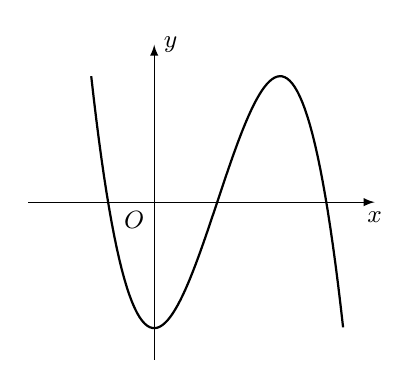
\begin{tikzpicture}[>=latex, scale=0.8]
    % Hệ trục tọa độ
    \draw[->] (-2,0) -- (3.5,0) node[below] {\small $x$};
    \draw[->] (0,-2.5) -- (0,2.5) node[right] {\small $y$};
    \node[below left] at (0,0) {\small $O$};
    
    % Đồ thị hàm bậc 4 trùng phương: y = -x^4 + x^2 - 2
    \draw[thick, samples=100, domain=-1:3] 
        plot (\x, {-\x*\x*\x +3*\x*\x - 2});
    
   
\end{tikzpicture}
\end{center}

}{
    \begin{tasks}(4)
        \task \( y = x^4 - x^2 - 2 \)
        \task \( y = -x^4 + x^2 - 2 \)
        \task \( y = -x^3 + 3x^2 - 2 \)
        \task \( y = x^3 - 3x^2 - 2 \)
    \end{tasks}
}

% --- CÂU 12 ---
\questionLinesManual{0}{12}{Đường cong trong hình vẽ bên là đồ thị của hàm số nào dưới đây?

\begin{center}
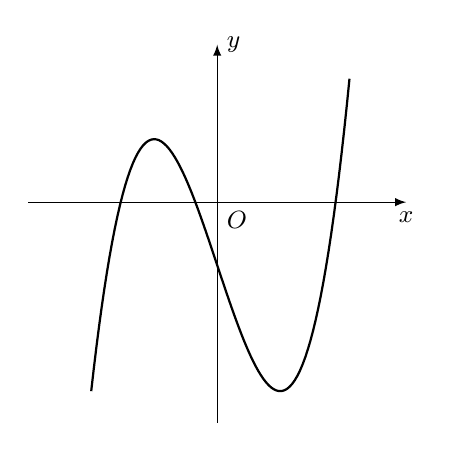
\begin{tikzpicture}[>=latex, scale=0.8]
    % Hệ trục tọa độ
    \draw[->] (-3,0) -- (3,0) node[below] {\small $x$};
    \draw[->] (0,-3.5) -- (0,2.5) node[right] {\small $y$};
    \node[below right] at (0,0) {\small $O$};
    
    % Đồ thị hàm bậc 3: y = x^3 - 3x - 1
    \draw[thick, samples=100, domain=-2:2.1] 
        plot (\x, {\x*\x*\x - 3*\x - 1});
\end{tikzpicture}
\end{center}

}{
    \begin{tasks}(4)
        \task \( y = x^3 - 3x - 1 \)
        \task \( y = x^4 - 3x^2 - 1 \)
        \task \( y = -x^3 - 3x - 1 \)
        \task \( y = -x^4 + x^2 - 1 \)
    \end{tasks}
}

% --- CÂU 13 ---
\questionLinesManual{0}{13}{Hình vẽ sau đây là đồ thị của một trong bốn hàm số cho ở các đáp án. Hỏi đó là hàm số nào?

\begin{center}
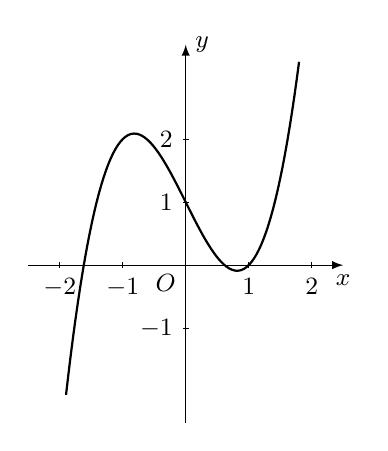
\begin{tikzpicture}[>=latex, scale=0.8]
    % Hệ trục tọa độ
    \draw[->] (-2.5,0) -- (2.5,0) node[below] {\small $x$};
    \draw[->] (0,-2.5) -- (0,3.5) node[right] {\small $y$};
    \node[below left] at (0,0) {\small $O$};
    \foreach \x in {-2,-1,1,2} {
         \draw (\x,0.05) -- (\x,-0.05)  node[below] {\small $\x$};
    }
    \foreach \y in {-1,1,2} {
          \draw (0.05,\y) -- (-0.05,\y)   node[left] {\small $\y$};
    }
    % Đồ thị hàm bậc 3: y = x^3 - 2x + 1
    \draw[thick, samples=100, domain=-1.9:1.8] 
        plot (\x, {\x*\x*\x - 2*\x + 1});
    
\end{tikzpicture}
\end{center}

}{
    \begin{tasks}(4)
        \task \( y = x^3 + 2x + 1 \)
        \task \( y = x^3 - 2x^2 + 1 \)
        \task \( y = x^3 - 2x + 1 \)
        \task \( y = -x^3 + 2x + 1 \)
    \end{tasks}
}

% --- CÂU 14 ---
\questionLinesManual{0}{14}{Đường cong trong hình vẽ bên là đồ thị của hàm số nào sau đây?

\begin{center}
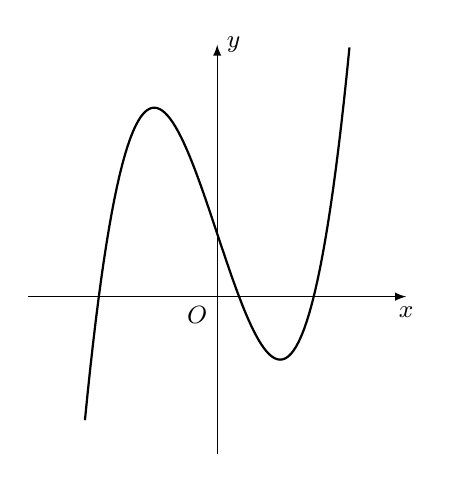
\begin{tikzpicture}[>=latex, scale=0.8]
    % Hệ trục tọa độ
    \draw[->] (-3,0) -- (3,0) node[below] {\small $x$};
    \draw[->] (0,-2.5) -- (0,4) node[right] {\small $y$};
    \node[below left] at (0,0) {\small $O$};
    
    % Đồ thị hàm bậc 3: y = -x^3 + 3x + 1
    \draw[thick, samples=100, domain=-2.1:2.1] 
        plot (\x, {\x*\x*\x - 3*\x + 1});
\end{tikzpicture}
\end{center}

}{
    \begin{tasks}(4)
        \task \( y = -x^3 + 3x + 1 \)
        \task \( y = x^4 - x^2 + 1 \)
        \task \( y = -x^2 + x - 1 \)
        \task \( y = x^3 - 3x + 1 \)
    \end{tasks}
}

% --- CÂU 15 ---
\questionLinesManual{0}{15}{Đồ thị của hàm số nào dưới đây có dạng đường cong như hình bên?

\begin{center}
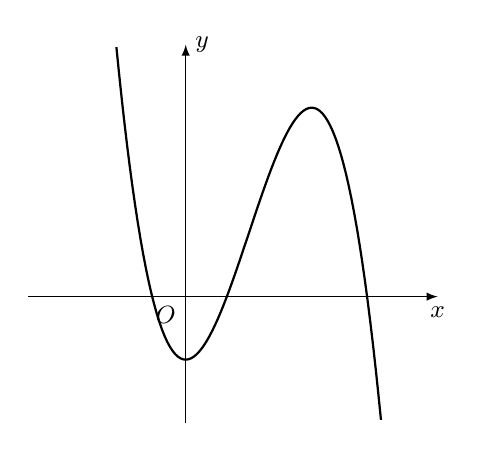
\begin{tikzpicture}[>=latex, scale=0.8]
    % Hệ trục tọa độ
    \draw[->] (-2.5,0) -- (4,0) node[below] {\small $x$};
    \draw[->] (0,-2) -- (0,4) node[right] {\small $y$};
    \node[below left] at (0,0) {\small $O$};
    
    \draw[thick, samples=100, domain=-1.1:3.1] 
        plot (\x, {(-\x*\x*\x +3*\x*\x - 1)});
\end{tikzpicture}
\end{center}

}{
    \begin{tasks}(4)
        \task \( y = x^3 - 3x^2 - 1 \)
        \task \( y = \dfrac{x^2 - 3x + 1}{x - 1} \)
        \task \( y = -x^3 + 3x^2 - 1 \)
        \task \( y = \dfrac{x + 1}{x - 1} \)
    \end{tasks}
}

% --- CÂU 16 ---
\questionLinesManual{0}{16}{Đồ thị sau đây là của hàm số nào?

\begin{center}
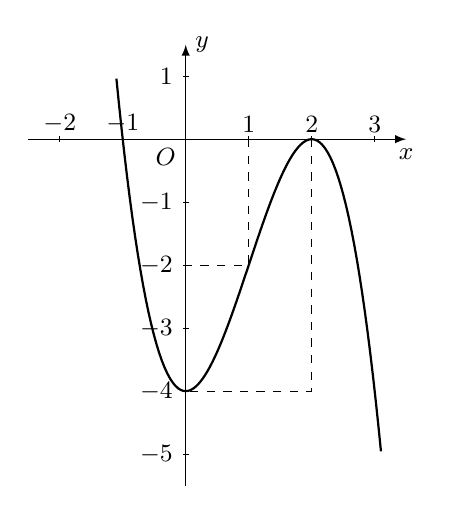
\begin{tikzpicture}[>=latex, scale=0.8]
    % Hệ trục tọa độ
    \draw[->] (-2.5,0) -- (3.5,0) node[below] {\small $x$};
    \draw[->] (0,-5.5) -- (0,1.5) node[right] {\small $y$};
    \node[below left] at (0,0) {\small $O$};
    
    % Đánh dấu các mốc
    \foreach \x in {-2,-1,1,2,3} {
         \draw (\x,0.05) -- (\x,-0.05)  node[above] {\small $\x$};
    }
    \foreach \y in {-5,-4,-3,-2,-1,1} {
          \draw (0.05,\y) -- (-0.05,\y)   node[left] {\small $\y$};
    }
    \draw[dashed] (1,0) -- (1,-2) -- (0,-2);
    \draw[dashed] (2,0) -- (2,-4) -- (0,-4);
    % Đồ thị hàm bậc 3: y = x^3 + 3x^2 - 4
    \draw[thick, samples=100, domain=-1.1:3.1] 
        plot (\x, {-\x*\x*\x + 3*\x*\x - 4});
\end{tikzpicture}
\end{center}

}{
    \begin{tasks}(4)
        \task \( y = -x^3 - 3x^2 - 4 \)
        \task \( y = x^3 + 3x^2 - 4 \)
        \task \( y = x^3 - 3x - 4 \)
        \task \( y = -x^3 + 3x^2 - 4 \)
    \end{tasks}
}

% --- CÂU 17 ---
\questionLinesManual{0}{17}{Đường cong ở hình sau là đồ thị của một trong bốn hàm số dưới đây. Hàm số đó là hàm số nào?

\begin{center}
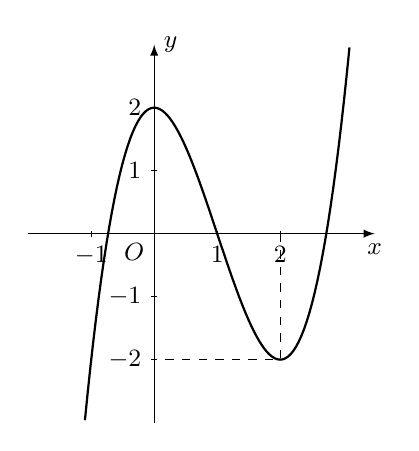
\begin{tikzpicture}[>=latex, scale=0.8]
    % Hệ trục tọa độ
    \draw[->] (-2,0) -- (3.5,0) node[below] {\small $x$};
    \draw[->] (0,-3) -- (0,3) node[right] {\small $y$};
    \node[below left] at (0,0) {\small $O$};
    
    % Đánh dấu các mốc
    \foreach \x in {-1,1,2} {
         \draw (\x,0.05) -- (\x,-0.05)  node[below] {\small $\x$};
    }
    \foreach \y in {-2,-1,1,2} {
          \draw (0.05,\y) -- (-0.05,\y)   node[left] {\small $\y$};
    }
    \draw[dashed] (2,0) -- (2,-2) -- (0,-2);
    % Đồ thị hàm bậc 3: y = x^3 - 3x + 2
    \draw[thick, samples=100, domain=-1.1:3.1] 
        plot (\x, {\x*\x*\x - 3*\x*\x + 2});
    
\end{tikzpicture}
\end{center}

}{
    \begin{tasks}(4)
        \task \( y = x^3 - 3x + 2 \)
        \task \( y = x^3 - 3x^2 + 2 \)
        \task \( y = x^3 - 6x + 2 \)
        \task \( y = -x^3 + 3x^2 + 2 \)
    \end{tasks}
}

% --- CÂU 18 ---
\questionLinesManual{0}{18}{Đồ thị hàm số nào sau đây có hình dạng như hình vẽ?

\begin{center}
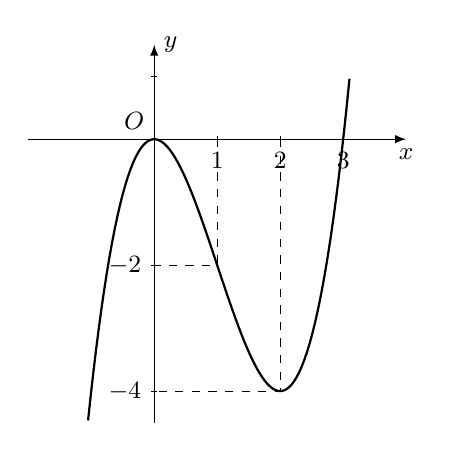
\begin{tikzpicture}[>=latex, scale=0.8]
    % Hệ trục tọa độ
    \draw[->] (-2,0) -- (4,0) node[below] {\small $x$};
    \draw[->] (0,-4.5) -- (0,1.5) node[right] {\small $y$};
    \node[above left] at (0,0) {\small $O$};
    
    % Đánh dấu các mốc
    \foreach \x in {1,2,3} {
         \draw (\x,0.05) -- (\x,-0.05)  node[below] {\small $\x$};
    }
    \foreach \y in {-4,-2,} {
          \draw (0.05,\y) -- (-0.05,\y)   node[left] {\small $\y$};
    }
    
    % Đồ thị hàm bậc 3: y = x^3 - 3x
    \draw[thick, samples=100, domain=-1.05:3.1] 
        plot (\x, {\x*\x*\x - 3*\x*\x});
    
    % Đánh dấu điểm cực trị
    \draw[dashed] (1,0) -- (1,-2)-- (0,-2);
    \draw[dashed] (2,0) -- (2,-4)-- (0,-4);
\end{tikzpicture}
\end{center}

}{
    \begin{tasks}(4)
        \task \( y = x^3 + 3x \)
        \task \( y = x^3 - 3x \)
        \task \( y = x^3 - 3x^2 \)
        \task \( y = x^3 + 3x^2 \)
    \end{tasks}
}

% --- CÂU 19 ---
\questionLinesManual{0}{19}{Đường cong ở hình sau là đồ thị của một trong bốn hàm số dưới đây. Hàm số đó là hàm số nào?

\begin{center}
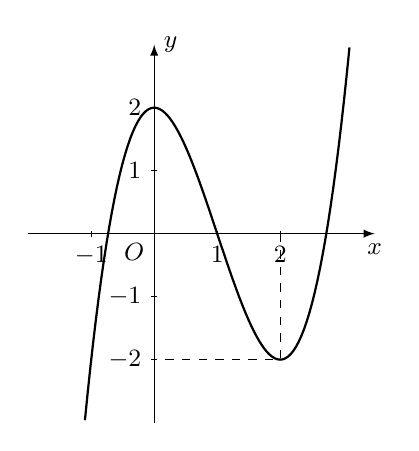
\begin{tikzpicture}[>=latex, scale=0.8]
    % Hệ trục tọa độ
    \draw[->] (-2,0) -- (3.5,0) node[below] {\small $x$};
    \draw[->] (0,-3) -- (0,3) node[right] {\small $y$};
    \node[below left] at (0,0) {\small $O$};
    
    % Đánh dấu các mốc
    \foreach \x in {-1,1,2} {
         \draw (\x,0.05) -- (\x,-0.05)  node[below] {\small $\x$};
    }
    \foreach \y in {-2,-1,1,2} {
          \draw (0.05,\y) -- (-0.05,\y)   node[left] {\small $\y$};
    }
    \draw[dashed] (2,0) -- (2,-2) -- (0,-2);
    % Đồ thị hàm bậc 3: y = x^3 - 3x + 2
    \draw[thick, samples=100, domain=-1.1:3.1] 
        plot (\x, {\x*\x*\x - 3*\x*\x + 2});
    
\end{tikzpicture}
\end{center}

}{
    \begin{tasks}(4)
        \task \( y = x^3 - 3x + 2 \)
        \task \( y = x^3 - 3x^2 + 2 \)
        \task \( y = x^3 - 6x + 2 \)
        \task \( y = -x^3 + 3x^2 + 2 \)
    \end{tasks}
}

% --- CÂU 20 ---
\questionLinesManual{0}{20}{Hàm số nào dưới đây có đồ thị là đường cong trong hình vẽ bên?

\begin{center}
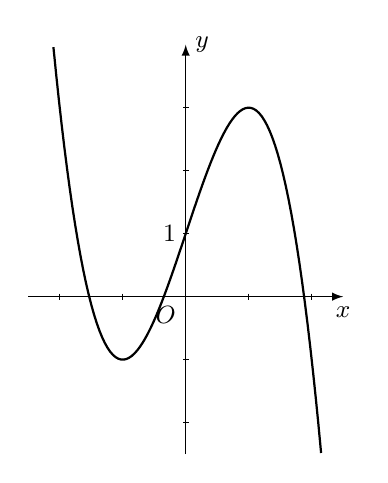
\begin{tikzpicture}[>=latex, scale=0.8]
    % Hệ trục tọa độ
    \draw[->] (-2.5,0) -- (2.5,0) node[below] {\small $x$};
    \draw[->] (0,-2.5) -- (0,4) node[right] {\small $y$};
    \node[below left] at (0,0) {\small $O$};
    
    % Đánh dấu các mốc
    \foreach \x in {-2,-1,1,2} {
         \draw (\x,0.05) -- (\x,-0.05)  ;
    }
    \foreach \y in {-2,-1,1,2,3} {
          \draw (0.05,\y) -- (-0.05,\y)  ;
    }
    
    % Đồ thị hàm bậc 3: y = -x^3 + 3x + 1
    \draw[thick, samples=100, domain=-2.1:2.15] 
        plot (\x, {-\x*\x*\x + 3*\x + 1});
    \node[left] at (0,1) {\small $1$};
\end{tikzpicture}
\end{center}

}{
    \begin{tasks}(4)
        \task \( y = -x^3 + 3x + 1 \)
        \task \( y = -x^2 + x - 1 \)
        \task \( y = x^3 - 3x + 1 \)
        \task \( y = x^4 - x^2 + 1 \)
    \end{tasks}
}

% --- CÂU 21 ---
\questionLinesManual{0}{21}{Đường cong hình bên dưới là đồ thị hàm số nào sau đây?

\begin{center}
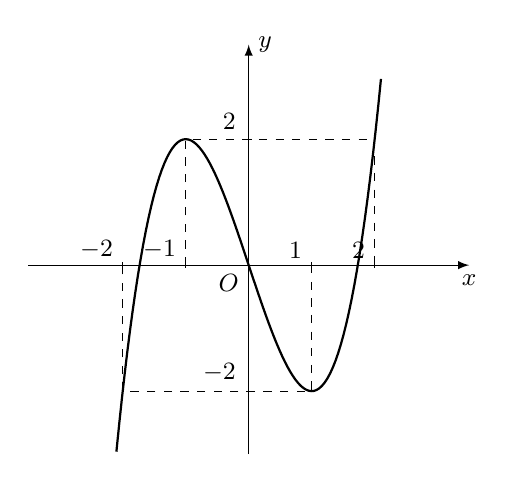
\begin{tikzpicture}[>=latex, scale=0.8]
    % Hệ trục tọa độ
    \draw[->] (-3.5,0) -- (3.5,0) node[below] {\small $x$};
    \draw[->] (0,-3) -- (0,3.5) node[right] {\small $y$};
    \node[below left] at (0,0) {\small $O$};
    
    % Đánh dấu các mốc
    \foreach \x in {-2,-1,1,2} {
         \draw (\x,0.05) -- (\x,-0.05)  node[above left] {\small $\x$};
    }
    \foreach \y in {-2,2} {
          \draw (0.05,\y) -- (-0.05,\y)   node[above left] {\small $\y$};
    }
    
    % Đồ thị hàm bậc 3: y = x^3 - 3x
    \draw[thick, samples=100, domain=-2.1:2.1] 
        plot (\x, {\x*\x*\x - 3*\x});
    
    % Đánh dấu điểm cực trị
    \draw[dashed] (-1,0) -- (-1,2) -- (2,2) --(2,0);
    \draw[dashed] (1,0) -- (1,-2) -- (-2,-2) --(-2,0);
\end{tikzpicture}
\end{center}

}{
    \begin{tasks}(4)
        \task \( y = x^3 - 3x^2 + 2 \)
        \task \( y = -x^3 + 2x \)
        \task \( y = x^3 + 3x^2 \)
        \task \( y = x^3 - 3x \)
    \end{tasks}
}

% --- CÂU 22 ---
\questionLinesManual{0}{22}{Cho hàm số bậc ba \( y = f(x) \) có đồ thị như hình vẽ. Công thức của hàm số bậc ba đã cho là:

\begin{center}
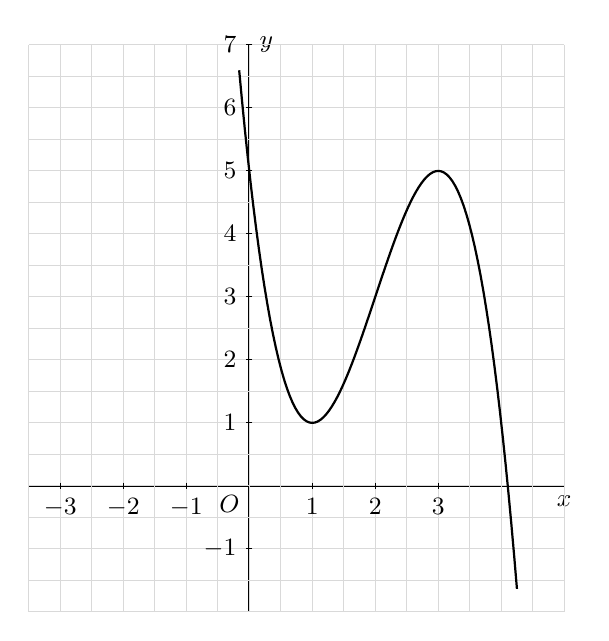
\begin{tikzpicture}[>=latex, scale=0.8]
\draw[thick] (-3.5,0) -- (5,0) node[below] {\small $x$};
    \draw[thick] (0,-2) -- (0,7) node[right] {\small $y$};
    \node[below left] at (0,0) {\small $O$};
    \draw[color=gray!30, thin, step=0.5] (-3.5,-2) grid (5,7);
    % Đánh dấu các mốc
    \foreach \x in {-3,-2,-1,1,2,3} {
        \draw (\x,0.05) -- (\x,-0.05) node[below] {\small $\x$};
    }
    \foreach \y in {-1,1,2,3,4,5,6,7} {
        \draw (0.05,\y) -- (-0.05,\y) node[left] {\small $\y$};
    }
    
    % Đồ thị hàm bậc 3: y = -x^3 + 6x^2 - 9x + 5
    \draw[thick, samples=100, domain=-0.16:4.25] 
        plot (\x, {-\x*\x*\x + 6*\x*\x - 9*\x + 5});
\end{tikzpicture}  
\end{center}

}{
    \begin{tasks}(4)
        \task \( y = x^3 - 5x + 5 \)
        \task \( y = -x^3 + 6x^2 + 9x + 5 \)
        \task \( y = -x^3 + 6x^2 - 9x + 5 \)
        \task \( y = x^3 - 2x^2 - 3x + 5 \)
    \end{tasks}
}

% --- CÂU 23 ---
\questionLinesManual{0}{23}{Đường cong ở hình sau là đồ thị của hàm số nào?

\begin{center}
\begin{tikzpicture}[>=latex, scale=0.8]
    % Hệ trục tọa độ
    \draw[->] (-3,0) -- (4,0) node[below] {\small $x$};
    \draw[->] (0,-5) -- (0,3.5) node[right] {\small $y$};
    \node[below left] at (0,0) {\small $O$};
    
    % Đồ thị hàm bậc 3: y = -x^3 + 3x^2 - 4
    \draw[thick, samples=100, domain=-1.3:3.1] 
        plot (\x, {-\x*\x*\x + 3*\x*\x - 4});
    
    % Đánh dấu điểm cực trị
    \draw[dashed] (0,0) -- (0,-4);
    \draw[dashed] (2,0) -- (2,0);
    \node[below left] at (-1,0) {\small $-1$};
    \node[above] at (2,0) {\small $2$};
    \node[left] at (0,-4) {\small $-4$};
\end{tikzpicture}
\end{center}

}{
    \begin{tasks}(4)
        \task \( y = -x^3 + 3x^2 - 4 \)
        \task \( y = x^3 - 4 \)
        \task \( y = x^2 - 4 \)
        \task \( y = -x^2 - 4 \)
    \end{tasks}
}

% --- CÂU 24 ---
\questionLinesManual{0}{24}{Đồ thị hàm số nào sau đây có dạng như hình vẽ?

\begin{center}
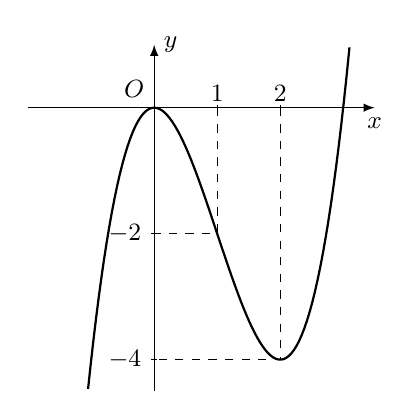
\begin{tikzpicture}[>=latex, scale=0.8]
    % Hệ trục tọa độ
    \draw[->] (-2,0) -- (3.5,0) node[below] {\small $x$};
    \draw[->] (0,-4.5) -- (0,1) node[right] {\small $y$};
    \node[above left] at (0,0) {\small $O$};
    
    % Đánh dấu các mốc
    \foreach \x in {1,2} {
         \draw (\x,0.05) -- (\x,-0.05)  node[above] {\small $\x$};
    }
    \foreach \y in {-4,-2} {
          \draw (0.05,\y) -- (-0.05,\y)   node[left] {\small $\y$};
    }
    
    % Đồ thị hàm bậc 3: y = -x^3 + 3x
    \draw[thick, samples=100, domain=-1.05:3.1] 
        plot (\x, {\x*\x*\x - 3*\x*\x});
    
    % Đánh dấu điểm cực trị
    \draw[dashed] (1,0) -- (1,-2) -- (0,-2);
    \draw[dashed] (2,0) -- (2,-4) -- (0,-4);
\end{tikzpicture}

\end{center}

}{
    \begin{tasks}(4)
        \task \( y = x^3 - 3x^2 \)
        \task \( y = x^3 + 3x \)
        \task \( y = -x^3 + 3x^2 \)
        \task \( y = -x^3 + 3x \)
    \end{tasks}
}

% --- CÂU 25 ---
\questionLinesManual{0}{25}{Đường cong hình bên là đồ thị của một trong bốn hàm số dưới đây. Hàm số đó là hàm số nào?

\begin{center}
\begin{tikzpicture}[>=latex, scale=0.8]
    % Hệ trục tọa độ
    \draw[->] (-3.5,0) -- (3.5,0) node[below] {\small $x$};
    \draw[->] (0,-2.5) -- (0,5) node[right] {\small $y$};
    \node[below left] at (0,0) {\small $O$};
    
    % Đánh dấu các mốc
    \foreach \x in {-2,-1,1,2} {
         \draw (\x,0.05) -- (\x,-0.05)  ;
    }
    \foreach \y in {-1,1,2,3,4} {
          \draw (0.05,\y) -- (-0.05,\y)  ;
    }
    
    % Đồ thị hàm bậc 3: y = x^3 - 3x + 2
    \draw[thick, samples=100, domain=-2.2:2.1] 
        plot (\x, {\x*\x*\x - 3*\x + 2});
\end{tikzpicture}
\end{center}

}{
    \begin{tasks}(4)
        \task \( y = -x^3 + 3x + 2 \)
        \task \( y = x^3 + x^2 + 1 \)
        \task \( y = x^3 - 3x + 2 \)
        \task \( y = x^2 + 1 \)
    \end{tasks}
}

% --- CÂU 26 ---
\questionLinesManual{0}{26}{Hình vẽ sau đây là đồ thị của một trong bốn hàm số cho ở các đáp án. Hỏi đó là hàm số nào?

\begin{center}
\begin{tikzpicture}[>=latex, scale=0.8]
    % Hệ trục tọa độ
    \draw[->] (-3.5,0) -- (3.5,0) node[below] {\small $x$};
    \draw[->] (0,-2) -- (0,3) node[right] {\small $y$};
    \node[below left] at (0,0) {\small $O$};
    
    % Đánh dấu các mốc
    \foreach \x in {-2,-1,1,2} {
         \draw (\x,0.05) -- (\x,-0.05)  node[below] {\small $\x$};
    }
    \foreach \y in {1,2} {
          \draw (0.05,\y) -- (-0.05,\y)   node[left] {\small $\y$};
    }
    
    % Đồ thị hàm bậc 3: y = x^3 - 2x + 1
    \draw[thick, samples=100, domain=-1.87:1.75] 
        plot (\x, {\x*\x*\x - 2*\x + 1});
\end{tikzpicture}
\end{center}

}{
    \begin{tasks}(4)
        \task \( y = x^3 + 2x + 1 \)
        \task \( y = x^3 - 2x^2 + 1 \)
        \task \( y = x^3 - 2x + 1 \)
        \task \( y = -x^3 + 2x + 1 \)
    \end{tasks}
}

% --- CÂU 27 ---
\questionLinesManual{0}{27}{Hình vẽ sau đây là đồ thị hàm số nào?

\begin{center}
\begin{tikzpicture}[>=latex, scale=0.8]
    % Hệ trục tọa độ
    \draw[->] (-3.5,0) -- (3.5,0) node[below] {\small $x$};
    \draw[->] (0,-2.5) -- (0,2.5) node[right] {\small $y$};
    \node[below left] at (0,0) {\small $O$};
    
    % Đánh dấu các mốc
    \foreach \x in {-3,-2,-1,1,2} {
         \draw (\x,0.05) -- (\x,-0.05)  node[below] {\small $\x$};
    }
    \foreach \y in {-2,-1,1,2} {
          \draw (0.05,\y) -- (-0.05,\y)   node[left] {\small $\y$};
    }
    
    % Đồ thị hàm bậc 3: y = x^3 - 2x^2 + 1
    \draw[thick, samples=100, domain=-1.05:2.25] 
        plot (\x, {\x*\x*\x - 2*\x*\x + 1});
   
\end{tikzpicture}
\end{center}

}{
    \begin{tasks}(4)
        \task \( y = x^3 - 2x + 1 \)
        \task \( y = x^3 - 2x^2 + 1 \)
        \task \( y = -x^3 + 2x^2 + 1 \)
        \task \( y = x^3 + 2x^2 + 1 \)
    \end{tasks}
}

% --- CÂU 28 ---
\questionLinesManual{0}{28}{Cho hàm số bậc ba \( y = f(x) \) có bảng biến thiên như sau:

\begin{center}
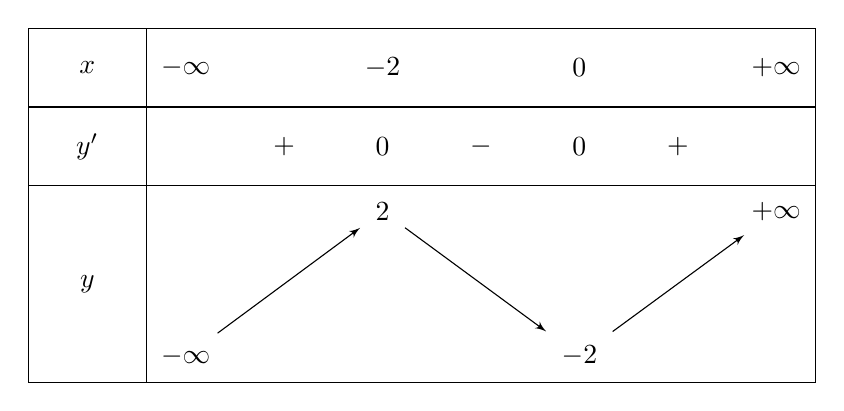
\begin{tikzpicture}
    \tkzTabInit[lgt=1.5, espcl=2.5]
    {$x$ /1, $y'$ /1, $y$ /2.5}
    {$-\infty$, $-2$, $0$, $+\infty$}
    \tkzTabLine{, +, 0, -, 0, +, }
    \tkzTabVar{-/ $-\infty$ / , +/ $2$ / , -/ $-2$ / , +/ $+\infty$ /}
\end{tikzpicture}
\end{center}

Khẳng định nào sau đây đúng?}{
    \begin{tasks}(4)
        \task \( f(x) = \dfrac{x^3}{3} + x^2 - 2 \)
        \task \( f(x) = x^3 + 3x^2 - 2 \)
        \task \( f(x) = -x^3 + 3x^2 - 2 \)
        \task \( f(x) = x^3 + 3x - 2 \)
    \end{tasks}
}

% --- CÂU 29 ---
\questionLinesManual{0}{29}{Hình vẽ sau là bảng biến thiên của hàm số nào dưới đây?

\begin{center}
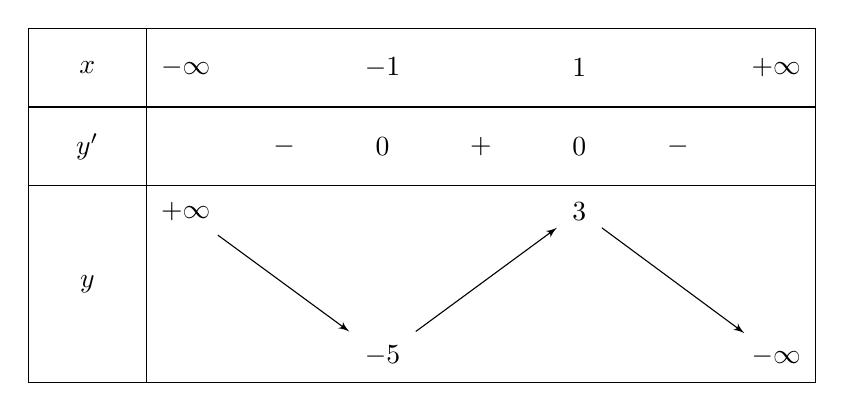
\begin{tikzpicture}
    \tkzTabInit[lgt=1.5, espcl=2.5]
    {$x$ /1, $y'$ /1, $y$ /2.5}
    {$-\infty$, $-1$, $1$, $+\infty$}
    \tkzTabLine{, -, 0, +, 0, -, }
    \tkzTabVar{+/ $+\infty$ / , -/ $-5$ / , +/ $3$ / , -/ $-\infty$ /}
\end{tikzpicture}
\end{center}

}{
    \begin{tasks}(4)
        \task \( y = -2x^4 + x^2 - 1 \)
        \task \( y = \dfrac{-2x + 7}{x + 3} \)
        \task \( y = -2x^2 + x - 1 \)
        \task \( y = -2x^3 + 6x - 1 \)
    \end{tasks}
}

% --- CÂU 30 ---
\questionLinesManual{0}{30}{Cho hàm số bậc ba \( y = f(x) \) có đồ thị là đường cong trong hình dưới đây:

\begin{center}
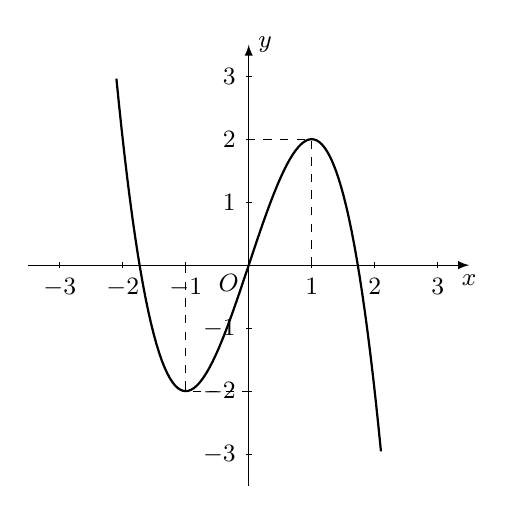
\begin{tikzpicture}[>=latex, scale=0.8]
    % Hệ trục tọa độ
    \draw[->] (-3.5,0) -- (3.5,0) node[below] {\small $x$};
    \draw[->] (0,-3.5) -- (0,3.5) node[right] {\small $y$};
    \node[below left] at (0,0) {\small $O$};
    
    % Đánh dấu các mốc
    \foreach \x in {-3,-2,-1,1,2,3} {
         \draw (\x,0.05) -- (\x,-0.05)  node[below] {\small $\x$};
    }
    \foreach \y in {-3,-2,-1,1,2,3} {
          \draw (0.05,\y) -- (-0.05,\y)   node[left] {\small $\y$};
    }
    
    % Đồ thị hàm bậc 3: y = x^3 - 3x + 1
    \draw[thick, samples=100, domain=-2.1:2.1] 
        plot (\x, {-\x*\x*\x + 3*\x});
    \draw[dashed] (1,0) -- (1,2)--(0,2);
    \draw[dashed] (-1,0) -- (-1,-2) -- (0,-2);
    
\end{tikzpicture}
\end{center}

Số nghiệm thực của phương trình \( f(x) = 3 \) là}{
    \begin{tasks}(4)
        \task $3$
        \task $0$
        \task $2$
        \task $1$
    \end{tasks}
}

% --- CÂU 31 ---
\questionLinesManual{0}{31}{Cho hàm số \( y = f(x) = ax^3 + bx^2 + cx + d \) (\( a \neq 0 \)) có đồ thị như hình vẽ.

\begin{center}
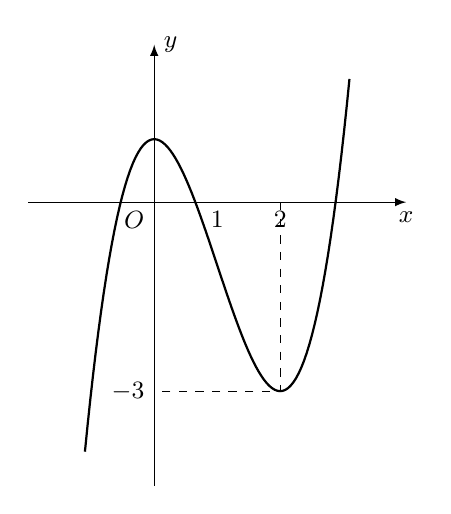
\begin{tikzpicture}[>=latex, scale=0.8]
    % Hệ trục tọa độ
    \draw[->] (-2,0) -- (4,0) node[below] {\small $x$};
    \draw[->] (0,-4.5) -- (0,2.5) node[right] {\small $y$};
    \node[below left] at (0,0) {\small $O$};
    
    
    % Đồ thị hàm bậc 3: y = x^3 - 3x
    \draw[thick, samples=100, domain=-1.1:3.1] 
        plot (\x, {\x*\x*\x - 3*\x*\x + 1});
    
    % Đánh dấu điểm cực trị
    \draw[dashed] (2,0) -- (2,-3) -- (0,-3);
    \node[below] at (1,0) {\small $1$};
    \node[below] at (2,0) {\small $2$};
    \node[left] at (0,-3) {\small $-3$};
\end{tikzpicture}
\end{center}

Số nghiệm của phương trình \( f(x) = -2 \) là}{
    \begin{tasks}(4)
        \task $2$
        \task $0$
        \task $1$
        \task $3$
    \end{tasks}
}

% --- CÂU 32 ---
\questionLinesManual{0}{32}{Cho hàm số \( y = f(x) \) liên tục trên \( \mathbb{R} \) và có đồ thị như hình vẽ.

\begin{center}
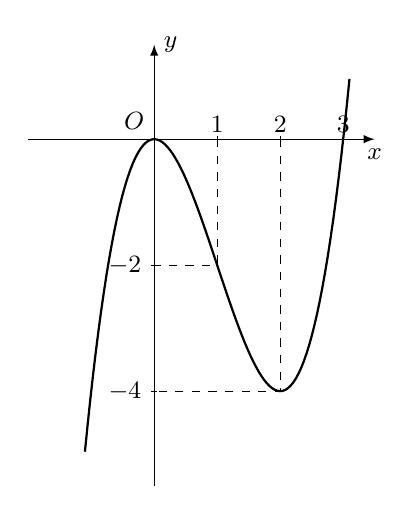
\begin{tikzpicture}[>=latex, scale=0.8]
    % Hệ trục tọa độ
    \draw[->] (-2,0) -- (3.5,0) node[below] {\small $x$};
    \draw[->] (0,-5.5) -- (0,1.5) node[right] {\small $y$};
    \node[above left] at (0,0) {\small $O$};
    
    % Đánh dấu các mốc
    \foreach \x in {1,2,3} {
         \draw (\x,0.05) -- (\x,-0.05)  node[above] {\small $\x$};
    }
    \foreach \y in {-4,-2} {
          \draw (0.05,\y) -- (-0.05,\y)   node[left] {\small $\y$};
    }
    
    % Đồ thị hàm bậc 3: y = x^3 - 3x
    \draw[thick, samples=100, domain=-1.1:3.1] 
        plot (\x, {\x*\x*\x - 3*\x*\x});
    
    % Đánh dấu điểm cực trị
    \draw[dashed] (2,0) -- (2,-4) -- (0,-4);
    \draw[dashed] (1,0) -- (1,-2)-- (0,-2);
    
    
\end{tikzpicture}
\end{center}

Phương trình \( f(x) = 0 \) có bao nhiêu nghiệm thực phân biệt?}{
    \begin{tasks}(4)
        \task $2$
        \task $1$
        \task $3$
        \task $0$
    \end{tasks}
}

% --- CÂU 33 ---
\questionLinesManual{0}{33}{Cho hàm số \( y = f(x) \) có đồ thị là đường cong trong hình dưới đây.

\begin{center}
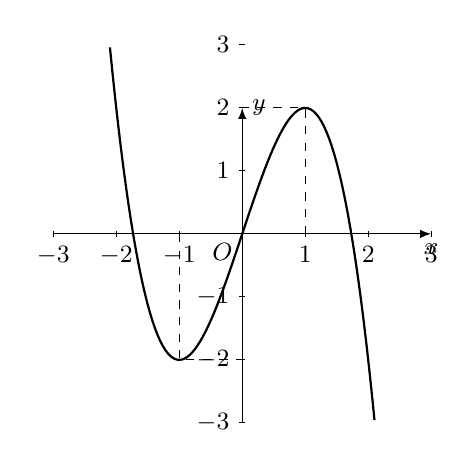
\begin{tikzpicture}[>=latex, scale=0.8]
    % Hệ trục tọa độ
    \draw[->] (-3,0) -- (3,0) node[below] {\small $x$};
    \draw[->] (0,-3) -- (0,2) node[right] {\small $y$};
    \node[below left] at (0,0) {\small $O$};
    
    % Đánh dấu các mốc
    \foreach \x in {-3,-2,-1,1,2,3} {
         \draw (\x,0.05) -- (\x,-0.05)  node[below] {\small $\x$};
    }
    \foreach \y in {-3,-2,-1,1,2,3} {
          \draw (0.05,\y) -- (-0.05,\y)   node[left] {\small $\y$};
    }
    
    % Đồ thị hàm bậc 3: y = x^3 - 3x + 1
    \draw[thick, samples=100, domain=-2.1:2.1] 
        plot (\x, {-\x*\x*\x + 3*\x});
    \draw[dashed] (1,0) -- (1,2)--(0,2);
    \draw[dashed] (-1,0) -- (-1,-2) -- (0,-2);
    
\end{tikzpicture}
\end{center}

Số giao điểm của đồ thị hàm số với trục tung là}{
    \begin{tasks}(4)
        \task $0$
        \task $3$
        \task $1$
        \task $O(0;0)$
    \end{tasks}
}

% --- CÂU 34 ---
\questionLinesManual{0}{34}{Cho hàm số \( y = ax^3 + 3x - d \) (\( a, d \in \mathbb{R} \)) có đồ thị là đường cong trong hình vẽ.

\begin{center}
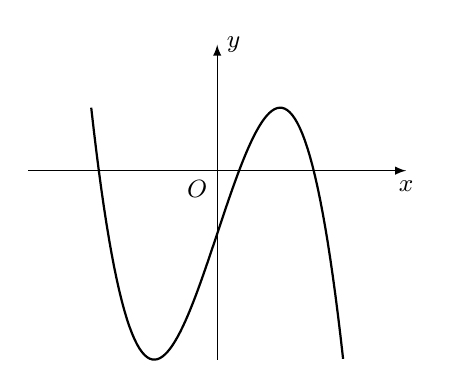
\begin{tikzpicture}[>=latex, scale=0.8]
    % Hệ trục tọa độ
    \draw[->] (-3,0) -- (3,0) node[below] {\small $x$};
    \draw[->] (0,-3) -- (0,2) node[right] {\small $y$};
    \node[below left] at (0,0) {\small $O$};
    
    
    % Đồ thị hàm bậc 3: y = -x^3 + 3x + 2
    \draw[thick, samples=100, domain=-2:2] 
        plot (\x, {-\x*\x*\x + 3*\x -1});
\end{tikzpicture}
\end{center}

Khẳng định nào dưới đây đúng?}{
    \begin{tasks}(4)
        \task \( a < 0, d > 0 \)
        \task \( a < 0, d < 0 \)
        \task \( a > 0, d < 0 \)
        \task \( a > 0, d > 0 \)
    \end{tasks}
}

% --- CÂU 35 ---
\questionLinesManual{0}{35}{Cho hàm số \( y = ax^3 + bx^2 + cx + d \) có đồ thị như hình vẽ. Khẳng định nào dưới đây đúng?

\begin{center}
\begin{tikzpicture}[>=latex, scale=0.8]
    % Hệ trục tọa độ
    \draw[->] (-3.5,0) -- (3.5,0) node[below] {\small $x$};
    \draw[->] (0,-4.5) -- (0,4.5) node[right] {\small $y$};
    \node[below left] at (0,0) {\small $O$};   
    % Đồ thị hàm bậc 3: y = x^3 - 3x
    \draw[thick, samples=100, domain=-2:2] 
        plot (\x, {-\x*\x*\x + 3*\x-1});
   
\end{tikzpicture}
\end{center}

}{
    \begin{tasks}(2)
        \task Hàm số đã cho đồng biến trên khoảng \((-\infty; +\infty)\).
        \task \( a > 0, d < 0 \).
        \task \( a < 0, d > 0 \).
        \task Hàm số đã cho có hai điểm cực trị.
    \end{tasks}
}

% --- CÂU 37 ---
\questionLinesManual{0}{36}{Cho hàm số \( y = ax^3 + 3x + d \) (\( a, d \in \mathbb{R} \)) có đồ thị như hình bên. Mệnh đề nào dưới đây đúng?

\begin{center}
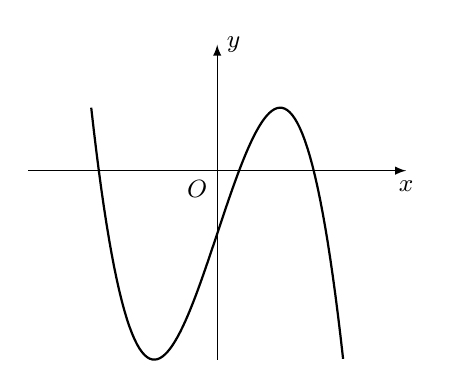
\begin{tikzpicture}[>=latex, scale=0.8]
    % Hệ trục tọa độ
    \draw[->] (-3,0) -- (3,0) node[below] {\small $x$};
    \draw[->] (0,-3) -- (0,2) node[right] {\small $y$};
    \node[below left] at (0,0) {\small $O$};   
    % Đồ thị hàm bậc 3: y = x^3 - 3x
    \draw[thick, samples=100, domain=-2:2] 
        plot (\x, {-\x*\x*\x + 3*\x-1});
   
\end{tikzpicture}
\end{center}

}{
    \begin{tasks}(4)
        \task \( a > 0, d > 0 \)
        \task \( a < 0, d > 0 \)
        \task \( a > 0, d < 0 \)
        \task \( a < 0, d < 0 \)
    \end{tasks}
}
% --- CÂU 36 ---
\questionLinesManual{0}{37}{Cho hàm số \( f(x) = ax^3 + bx^2 + cx + d \) (\( a, b, c, d \in \mathbb{R} \)) có bảng biến thiên như sau:

\begin{center}
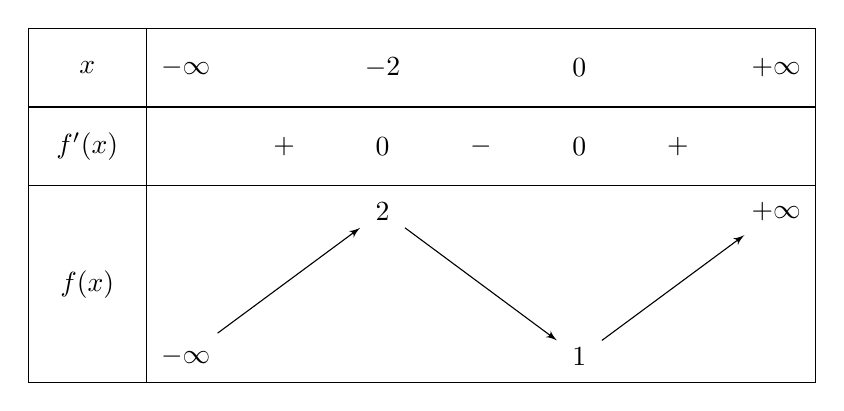
\begin{tikzpicture}
    \tkzTabInit[lgt=1.5, espcl=2.5]
    {$x$ /1, $f'(x)$ /1, $f(x)$ /2.5}
    {$-\infty$, $-2$, $0$, $+\infty$}
    \tkzTabLine{, +, 0, -, 0, +, }
    \tkzTabVar{-/ $-\infty$ / , +/ $2$ / , -/ $1$ / , +/ $+\infty$ /}
\end{tikzpicture}
\end{center}

Có bao nhiêu số dương trong các số \( a, b, c, d \)?}{
    \begin{tasks}(4)
        \task $2$
        \task $4$
        \task $1$
        \task $3$
    \end{tasks}
}



% --- CÂU 38 ---
\questionLinesManual{0}{38}{Cho hàm số \( y = ax^3 + bx^2 + cx + d \) (\( a, b, c, d \in \mathbb{R} \)) có đồ thị là đường cong trong hình bên. Có bao nhiêu số dương trong các số \( a, b, c, d \)?

\begin{center}

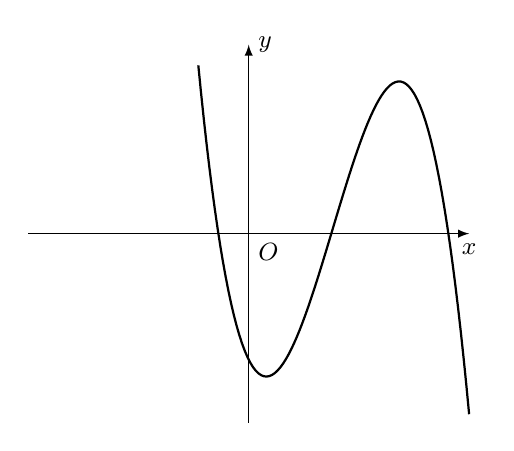
\begin{tikzpicture}[>=latex, scale=0.8]
    % Hệ trục tọa độ
    \draw[->] (-3.5,0) -- (3.5,0) node[below] {\small $x$};
    \draw[->] (0,-3) -- (0,3) node[right] {\small $y$};
    \node[below right] at (0,0) {\small $O$};
    
   
    % Đồ thị hàm bậc 3: y = x^3 - 3x
    \draw[thick, samples=100, domain=-0.8:3.5] 
        plot (\x, {-\x*\x*\x+4*\x*\x -2*\x -2});
  
\end{tikzpicture}
\end{center}

}{
    \begin{tasks}(4)
        \task $4$
        \task $1$
        \task $2$
        \task $3$
    \end{tasks}
}

% --- CÂU 39 ---
\questionLinesManual{0}{39}{Cho hàm số \( y = ax^3 + bx^2 + cx + d \) (\( a, b, c, d \in \mathbb{R} \)) có đồ thị là đường cong trong hình bên. Có bao nhiêu số dương trong các hệ số \( a, b, c, d \)?

\begin{center}
\begin{tikzpicture}[>=latex, scale=0.8]
    % Hệ trục tọa độ
    \draw[->] (-2,0) -- (5,0) node[below] {\small $x$};
    \draw[->] (0,-3) -- (0,5) node[right] {\small $y$};
    \node[below right] at (0,0) {\small $O$};
    
   
    % Đồ thị hàm bậc 3: y = x^3 - 3x
    \draw[thick, samples=100, domain=-0.35:4.35] 
        plot (\x, {-\x*\x*\x+6*\x*\x -8*\x +1});
  
\end{tikzpicture}
\end{center}

}{
    \begin{tasks}(4)
        \task $4$
        \task $3$
        \task $1$
        \task $2$
    \end{tasks}
}

% --- CÂU 40 ---
\questionLinesManual{0}{40}{Cho hàm số \( y = ax^3 + bx^2 + cx + d \) (\( a, b, c, d \in \mathbb{R} \)) có đồ thị là đường cong trong hình bên. Có bao nhiêu số dương trong các số \( a, b, c, d \)?

\begin{center}
\begin{tikzpicture}[>=latex, scale=0.8]
    % Hệ trục tọa độ
    \draw[->] (-6,0) -- (2,0) node[below] {\small $x$};
    \draw[->] (0,-3) -- (0,5) node[right] {\small $y$};
    \node[below right] at (0,0) {\small $O$};
    
   
    % Đồ thị hàm bậc 3: y = x^3 - 3x
    \draw[thick, samples=100, domain=-4.5:1.2] 
        plot (\x, {-0.5*(\x+4)*(\x+2)*(\x-1)});
  
\end{tikzpicture}
\end{center}

}{
    \begin{tasks}(4)
        \task $4$
        \task $2$
        \task $1$
        \task $3$
    \end{tasks}
}

% --- CÂU 41 ---
\questionLinesManual{0}{41}{Cho hàm số \( y = ax^3 + bx^2 + cx + d \) (\( a, b, c, d \in \mathbb{R} \)) có đồ thị là đường cong trong hình bên. Có bao nhiêu số dương trong các số \( a, b, c, d \)?

\begin{center}
\begin{tikzpicture}[>=latex, scale=0.8]
    % Hệ trục tọa độ
    \draw[->] (-6,0) -- (5,0) node[below] {\small $x$};
    \draw[->] (0,-3) -- (0,5) node[right] {\small $y$};
    \node[below right] at (0,0) {\small $O$};
    
   
    % Đồ thị hàm bậc 3: y = x^3 - 3x
    \draw[thick, samples=100, domain=-4.6:3.4] 
        plot (\x, {-0.2*(\x+4)*(\x+1)*(\x-3)});
  
\end{tikzpicture}
\end{center}

}{
    \begin{tasks}(4)
        \task $4$
        \task $2$
        \task $1$
        \task $3$
    \end{tasks}
}

% --- CÂU 42 ---
\questionLinesManual{0}{42}{Cho hàm số \( f(x) = ax^3 + bx^2 + cx + d \) (\( a, b, c, d \in \mathbb{R} \)) có bảng biến thiên như sau

\begin{center}
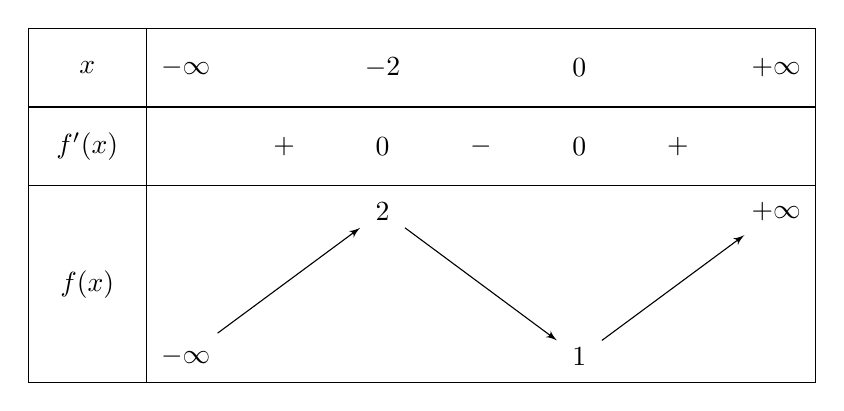
\begin{tikzpicture}
    \tkzTabInit[lgt=1.5, espcl=2.5]
    {$x$ /1, $f'(x)$ /1, $f(x)$ /2.5}
    {$-\infty$, $-2$, $0$, $+\infty$}
    \tkzTabLine{, +, 0, -, 0, +, }
    \tkzTabVar{-/ $-\infty$ / , +/ $2$ / , -/ $1$ / , +/ $+\infty$ /}
\end{tikzpicture}
\end{center}

Có bao nhiêu số dương trong các số \( a, b, c, d \)?}{
    \begin{tasks}(4)
        \task $2$
        \task $4$
        \task $1$
        \task $3$
    \end{tasks}
}

% --- CÂU 43 ---
\questionLinesManual{0}{43}{Cho hàm số \( f(x) = ax^3 + bx^2 + cx + d \) (\( a, b, c, d \in \mathbb{R} \)) có bảng biến thiên như sau:

\begin{center}
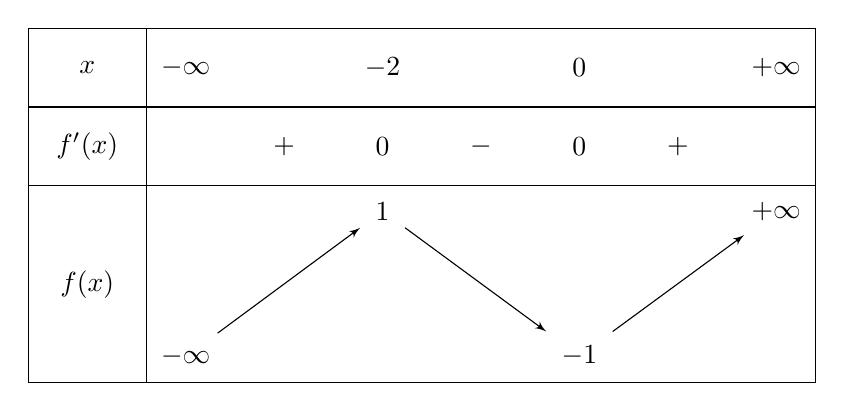
\begin{tikzpicture}
    \tkzTabInit[lgt=1.5, espcl=2.5]
    {$x$ /1, $f'(x)$ /1, $f(x)$ /2.5}
    {$-\infty$, $-2$, $0$, $+\infty$}
    \tkzTabLine{, +, 0, -, 0, +, }
    \tkzTabVar{-/ $-\infty$ / , +/ $1$ / , -/ $-1$ / , +/ $+\infty$ /}
\end{tikzpicture}
\end{center}

Có bao nhiêu số dương trong các số \( a, b, c, d \)?}{
    \begin{tasks}(4)
        \task $3$
        \task $4$
        \task $2$
        \task $1$
    \end{tasks}
}

% --- CÂU 44 ---
\questionLinesManual{0}{44}{Cho hàm số \( f(x) = ax^3 + bx^2 + cx + d \) (\( a, b, c, d \in \mathbb{R} \)) có bảng biến thiên như sau:

\begin{center}
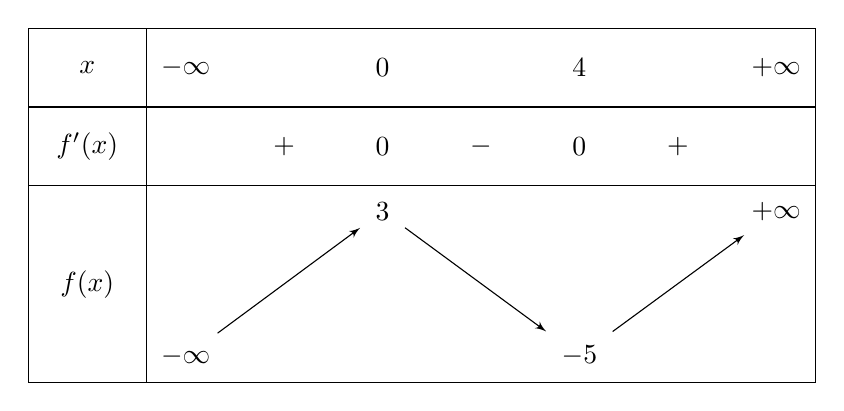
\begin{tikzpicture}
    \tkzTabInit[lgt=1.5, espcl=2.5]
    {$x$ /1, $f'(x)$ /1, $f(x)$ /2.5}
    {$-\infty$, $0$, $4$, $+\infty$}
    \tkzTabLine{, +, 0, -, 0, +, }
    \tkzTabVar{-/ $-\infty$ / , +/ $3$ / , -/ $-5$ / , +/ $+\infty$ /}
\end{tikzpicture}
\end{center}

Có bao nhiêu số dương trong các số \( a, b, c, d \)?}{
    \begin{tasks}(4)
        \task $2$
        \task $4$
        \task $1$
        \task $3$
    \end{tasks}
}

% --- CÂU 45 ---
\questionLinesManual{0}{45}{Cho hàm số \( f(x) = ax^3 + bx^2 + cx + d \) (\( a, b, c, d \in \mathbb{R} \)) có bảng biến thiên như sau:

\begin{center}
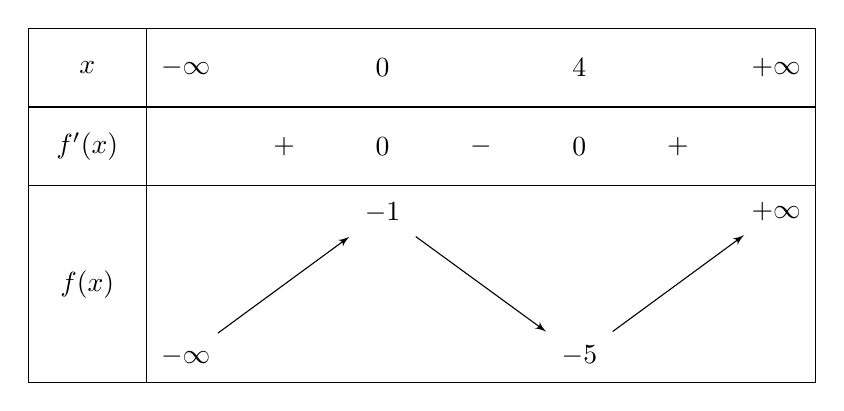
\begin{tikzpicture}
    \tkzTabInit[lgt=1.5, espcl=2.5]
    {$x$ /1, $f'(x)$ /1, $f(x)$ /2.5}
    {$-\infty$, $0$, $4$, $+\infty$}
    \tkzTabLine{, +, 0, -, 0, +, }
    \tkzTabVar{-/ $-\infty$ / , +/ $-1$ / , -/ $-5$ / , +/ $+\infty$ /}
\end{tikzpicture}
\end{center}

Có bao nhiêu số dương trong các số \( a, b, c, d \)?}{
    \begin{tasks}(4)
        \task $4$
        \task $2$
        \task $3$
        \task $1$
    \end{tasks}
}

% --- CÂU 46 ---
\questionLinesManual{0}{46}{Cho hàm số \( y = ax^3 + bx^2 + cx + d \) có đồ thị như hình vẽ bên. Mệnh đề nào dưới đây đúng?

\begin{center}
\begin{tikzpicture}[>=latex, scale=0.8]
    % Hệ trục tọa độ
    \draw[->] (-4,0) -- (5,0) node[below] {\small $x$};
    \draw[->] (0,-4) -- (0,5) node[right] {\small $y$};
    \node[below right] at (0,0) {\small $O$};
    
   
    % Đồ thị hàm bậc 3: y = x^3 - 3x
    \draw[thick, samples=100, domain=-2.55:4.5] 
        plot (\x, {-0.3*(\x+2)*(\x-1)*(\x-4)});
  
\end{tikzpicture}
\end{center}

}{
    \begin{tasks}(2)
        \task \( a < 0, b > 0, c > 0, d < 0 \)
        \task \( a < 0, b < 0, c > 0, d < 0 \)
        \task \( a > 0, b < 0, c < 0, d > 0 \)
        \task \( a < 0, b > 0, c < 0, d < 0 \)
    \end{tasks}
}

% --- CÂU 47 ---
\questionLinesManual{0}{47}{Cho hàm số \( y = ax^3 + bx^2 + cx + d \) (\( a \neq 0 \)) có đồ thị như hình vẽ dưới đây. Chọn khẳng định đúng về dấu của \( a, b, c, d \)?

\begin{center}
\begin{tikzpicture}[>=latex, scale=0.8]
    % Hệ trục tọa độ
    \draw[->] (-4,0) -- (5,0) node[below] {\small $x$};
    \draw[->] (0,-4) -- (0,5) node[right] {\small $y$};
    \node[below right] at (0,0) {\small $O$};
    
   
    % Đồ thị hàm bậc 3: y = x^3 - 3x
    \draw[thick, samples=100, domain=-2.55:4.5] 
        plot (\x, {0.3*(\x+2)*(\x-1)*(\x-4)});
  
\end{tikzpicture}
\end{center}

}{
    \begin{tasks}(2)
        \task \( a > 0, b > 0, d > 0, c > 0 \)
        \task \( a > 0, c > 0 > b, d < 0 \)
        \task \( a > 0, b > 0, c > 0, d > 0 \)
        \task \( a > 0, b < 0, c < 0, d > 0 \)
    \end{tasks}
}

% --- CÂU 48 ---
\questionLinesManual{0}{48}{Hàm số \( y = ax^3 + bx^2 + cx + d \) có đồ thị như hình vẽ bên dưới:

\begin{center}
\begin{tikzpicture}[>=latex, scale=0.8]
    % Hệ trục tọa độ
    \draw[->] (-5,0) -- (6,0) node[below] {\small $x$};
    \draw[->] (0,-4) -- (0,6) node[right] {\small $y$};
    \node[below right] at (0,0) {\small $O$};
    
   
    % Đồ thị hàm bậc 3: y = x^3 - 3x
    \draw[thick, samples=100, domain=-3.4:4.7] 
        plot (\x, {0.25*(\x+3)*(\x-1)*(\x-4)});
  
\end{tikzpicture}
\end{center}

Khẳng định nào là đúng?}{
    \begin{tasks}(2)
        \task \( a < 0, b < 0, c < 0, d < 0 \)
        \task \( a > 0, b > 0, c > 0, d < 0 \)
        \task \( a > 0, b > 0, c < 0, d > 0 \)
        \task \( a > 0, b < 0, c < 0, d > 0 \)
    \end{tasks}
}

% --- CÂU 49 ---
\questionLinesManual{0}{49}{Cho hàm số \( y = ax^3 + bx^2 + cx + d \) có đồ thị như hình bên. Trong các mệnh đề sau mệnh đề nào đúng?

\begin{center}
\begin{tikzpicture}[>=latex, scale=0.8]
    % Hệ trục tọa độ
    \draw[->] (-2,0) -- (5,0) node[below] {\small $x$};
    \draw[->] (0,-5) -- (0,2) node[right] {\small $y$};
    \node[below right] at (0,0) {\small $O$};
    
   
    % Đồ thị hàm bậc 3: y = x^3 - 3x
    \draw[thick, samples=100, domain=-1.8:4.2] 
        plot (\x, {0.4*(\x+1)*(\x-0.6)*(\x-4)});
  
\end{tikzpicture}
\end{center}

}{
    \begin{tasks}(2)
        \task \( ab < 0, bc > 0, cd < 0 \)
        \task \( ab < 0, bc < 0, cd > 0 \)
        \task \( ab > 0, bc > 0, cd < 0 \)
        \task \( ab > 0, bc > 0, cd > 0 \)
    \end{tasks}
}

% --- CÂU 50 ---
\questionLinesManual{0}{50}{Cho hàm số \( y = ax^3 + bx^2 + cx + d \) có đồ thị như hình dưới. Khẳng định nào sau đây đúng?

\begin{center}
\begin{tikzpicture}[>=latex, scale=0.8]
    % Hệ trục tọa độ
    \draw[->] (-5,0) -- (4,0) node[below] {\small $x$};
    \draw[->] (0,-5) -- (0,2) node[right] {\small $y$};
    \node[below left] at (0,0) {\small $O$};
    
   
    % Đồ thị hàm bậc 3: y = x^3 - 3x
    \draw[thick, samples=100, domain=-4.25:3.2] 
        plot (\x, {-0.2*(\x+4)*(\x-0.6)*(\x-2)});
  
\end{tikzpicture}
\end{center}

}{
    \begin{tasks}(2)
        \task \( a < 0, b < 0, c < 0, d < 0 \)
        \task \( a < 0, b > 0, c > 0, d > 0 \)
        \task \( a < 0, b > 0, c < 0, d > 0 \)
        \task \( a < 0, b > 0, c > 0, d < 0 \)
    \end{tasks}
}

% --- CÂU 51 ---
\questionLinesManual{0}{51}{Hàm số \( y = ax^3 + bx^2 + cx + d \) có đồ thị như hình vẽ bên dưới:

\begin{center}

\begin{tikzpicture}[>=latex, scale=0.8]
    % Hệ trục tọa độ
    \draw[->] (-2,0) -- (6,0) node[below] {\small $x$};
    \draw[->] (0,-4) -- (0,4) node[right] {\small $y$};
    \node[below right] at (0,0) {\small $O$};
    
   
    % Đồ thị hàm bậc 3: y = x^3 - 3x
    \draw[thick, samples=100, domain=-1.5:5.1] 
        plot (\x, {-0.25*(\x+1)*(\x-3)*(\x-4)});
  
\end{tikzpicture}
\end{center}

Khẳng định nào là đúng?}{
    \begin{tasks}(2)
        \task \( a < 0, b < 0, c < 0, d < 0 \)
        \task \( a > 0, b > 0, c > 0, d < 0 \)
        \task \( a > 0, b > 0, c > 0, d > 0 \)
        \task \( a > 0, b < 0, c > 0, d > 0 \)
    \end{tasks}
}

% --- CÂU 52 ---
\questionLinesManual{0}{52}{Tìm đồ thị hàm số \( y = f(x) \) được cho bởi một trong các phương án dưới đây, biết \( f(x) = (a - x)(b - x)^2 \) với \( a < b \).


}{
    \begin{tasks}(2)
        \task \(\begin{tikzpicture}[>=latex, scale=0.8]
    % Hệ trục tọa độ
    \draw[->] (-1,0) -- (4,0) node[below] {\small $x$};
    \draw[->] (0,-2) -- (0,2) node[right] {\small $y$};
    \node[below right] at (0,0) {\small $O$};
    
   
    % Đồ thị hàm bậc 3: y = x^3 - 3x
    \draw[thick, samples=100, domain=0.7:3.8] 
        plot (\x, {(1-\x)*(3-\x)*(3-\x)});
  
\end{tikzpicture}\)
        \task \(\begin{tikzpicture}[>=latex, scale=0.8]
    % Hệ trục tọa độ
    \draw[->] (-1,0) -- (4,0) node[below] {\small $x$};
    \draw[->] (0,-2) -- (0,2) node[right] {\small $y$};
    \node[below right] at (0,0) {\small $O$};
    
   
    % Đồ thị hàm bậc 3: y = x^3 - 3x
    \draw[thick, samples=100, domain=0.2:3.2] 
        plot (\x, {(1-\x)*(1-\x)*(3-\x)});
  
\end{tikzpicture}\)
        \task \(\begin{tikzpicture}[>=latex, scale=0.8]
   % Hệ trục tọa độ
    \draw[->] (-1,0) -- (4,0) node[below] {\small $x$};
    \draw[->] (0,-2) -- (0,2) node[right] {\small $y$};
    \node[below right] at (0,0) {\small $O$};
    
   
    % Đồ thị hàm bậc 3: y = x^3 - 3x
    \draw[thick, samples=100, domain=0.2:3.2] 
        plot (\x, {(1-\x)*(1-\x)*(-3+\x)});
  
\end{tikzpicture}\)
        \task \(\begin{tikzpicture}[>=latex, scale=0.8]
    % Hệ trục tọa độ
    \draw[->] (-1,0) -- (4,0) node[below] {\small $x$};
    \draw[->] (0,-2) -- (0,2) node[right] {\small $y$};
    \node[below right] at (0,0) {\small $O$};
    
   
    % Đồ thị hàm bậc 3: y = x^3 - 3x
    \draw[thick, samples=100, domain=0.7:3.8] 
        plot (\x, {(-1+\x)*(3-\x)*(3-\x)});
  
\end{tikzpicture}\)
    \end{tasks}
}

% --- CÂU 53 ---
\questionLinesManual{0}{53}{Cho đường cong \( (C) : y = ax^3 + bx^2 + cx + d \) có đồ thị như hình bên.

\begin{center}
\begin{tikzpicture}[>=latex, scale=0.8]
    % Hệ trục tọa độ
    \draw[->] (-3.5,0) -- (3.5,0) node[below] {\small $x$};
    \draw[->] (0,-3) -- (0,4) node[right] {\small $y$};
    \node[below right] at (0,0) {\small $O$};
   
    % Đồ thị hàm bậc 3: y = -x^3 + 3x^2 + 2
    \draw[thick, samples=100, domain=-3.5:2.5] 
        plot (\x, {0.2*(2*\x*\x*\x + 3*\x*\x - 12*\x)-1});
    \draw[dashed] (1,0) -- (1,-2.4);
    \draw[dashed] (-2,0) -- (-2,3);
    \node[above] at (1,0) {\small $1$};
    \node[below] at (-2,0) {\small $-2$};
\end{tikzpicture}
\end{center}

Khẳng định nào sau đây là đúng?}{
    \begin{tasks}(2)
        \task \( a > 0, b < 0, c < 0, d < 0 \)
        \task \( a > 0, b > 0, c < 0, d > 0 \)
        \task \( a < 0, b > 0, c > 0, d < 0 \)
        \task \( a > 0, b > 0, c < 0, d < 0 \)
    \end{tasks}
}

% --- CÂU 54 ---
\questionLinesManual{0}{54}{Cho hàm số \( y = f(x) = ax^3 + bx^2 + cx + d \) có đồ thị như hình vẽ ở bên. Mệnh đề nào sau đây đúng?

\begin{center}
\begin{tikzpicture}[>=latex, scale=0.8]
    % Hệ trục tọa độ
    \draw[->] (-1,0) -- (5,0) node[below] {\small $x$};
    \draw[->] (0,-1) -- (0,6) node[right] {\small $y$};
    \node[below right] at (0,0) {\small $O$};
   
    % Đồ thị hàm bậc 3: y = -x^3 + 3x^2 + 2
    \draw[thick, samples=100, domain=-0.2:4.1] 
        plot (\x, {\x*\x*\x - 6*\x*\x + 9*\x + 1});
    \draw[dashed] (1,0) -- (1,5) -- (0,5);
    \draw[dashed] (3,0) -- (3,1) -- (0,1);
    \node[below] at (1,0) {\small $1$};
    \node[below] at (3,0) {\small $3$};
    \node[left] at (0,1) {\small $1$};
    \node[left] at (0,5) {\small $5$};
\end{tikzpicture}
\end{center}

}{
    \begin{tasks}(2)
        \task \( a > 0, b > 0, c > 0, d > 0 \)
        \task \( a > 0, b > 0, c < 0, d > 0 \)
        \task \( a > 0, b < 0, c > 0, d > 0 \)
        \task \( a < 0, b < 0, c > 0, d < 0 \)
    \end{tasks}
}

% --- CÂU 55 ---
\questionLinesManual{0}{55}{Cho hàm số \( y = ax^3 + bx^2 + cx + d \) có đồ thị như hình vẽ. Tính \( S = a + b \)?

\begin{center}
\begin{tikzpicture}[>=latex, scale=0.8]
    % Hệ trục tọa độ
    \draw[->] (-2,0) -- (4,0) node[below] {\small $x$};
    \draw[->] (0,-3) -- (0,4) node[right] {\small $y$};
    \node[below right] at (0,0) {\small $O$};
    \foreach \x in {-1,1,2,3} {
         \draw (\x,0.05) -- (\x,-0.05) ;
    }
    \foreach \y in {-2,-1,1,2,3} {
          \draw (0.05,\y) -- (-0.05,\y)   ;
    }
    \draw[color=gray!30, thin, step=0.5] (-2,-3) grid (4,4);
    % Đồ thị hàm bậc 3: y = -x^3 + 3x^2 + 2
    \draw[thick, samples=100, domain=-1.05:3.15] 
        plot (\x, {\x*\x*\x - 3*\x*\x + 2});
   
\end{tikzpicture}
\end{center}

}{
    \begin{tasks}(4)
        \task \( S = -2 \)
        \task \( S = 0 \)
        \task \( S = 1 \)
        \task \( S = -1 \)
    \end{tasks}
}

% --- CÂU 56 ---
\questionLinesManual{0}{56}{Cho hàm số \( y = ax^3 + bx^2 + cx + d \) có đồ thị như hình vẽ bên. Mệnh đề nào dưới đây đúng?

\begin{center}
\begin{tikzpicture}[>=latex, scale=0.8]
    % Hệ trục tọa độ
    \draw[->] (-2,0) -- (4,0) node[below] {\small $x$};
    \draw[->] (0,-3) -- (0,4) node[right] {\small $y$};
    \node[below left] at (0,0) {\small $O$};
    
    % Đồ thị hàm bậc 3: y = -x^3 + 3x^2 + 2
    \draw[thick, samples=100, domain=-1.65:3.2] 
        plot (\x, {0.8*(\x+1)*(-\x+0.3)*(\x-3)-1});
   
\end{tikzpicture}
\end{center}

}{
    \begin{tasks}(2)
        \task \( a < 0, b < 0, c > 0, d < 0 \)
        \task \( a < 0, b > 0, c < 0, d < 0 \)
        \task \( a > 0, b < 0, c < 0, d > 0 \)
        \task \( a < 0, b > 0, c > 0, d < 0 \)
    \end{tasks}
}

% --- CÂU 57 ---
\questionLinesManual{0}{57}{Cho hàm số \( y = ax^3 + bx^2 + cx + d \) có đồ thị như hình vẽ. Trong các số \( a, b, c \) và \( d \) có bao nhiêu số dương?

\begin{center}
\begin{tikzpicture}[>=latex, scale=0.8]
    % Hệ trục tọa độ
    \draw[->] (-2,0) -- (4,0) node[below] {\small $x$};
    \draw[->] (0,-4) -- (0,3) node[right] {\small $y$};
    \node[below left] at (0,0) {\small $O$};
    
    % Đồ thị hàm bậc 3: y = -x^3 + 3x^2 + 2
    \draw[thick, samples=100, domain=-1.65:3.2] 
        plot (\x, {0.8*(\x+1)*(\x-0.3)*(\x-3)+1});
   
\end{tikzpicture}
\end{center}

}{
    \begin{tasks}(4)
        \task $1$
        \task $4$
        \task $3$
        \task $2$
    \end{tasks}
}

% --- CÂU 58 ---
\questionLinesManual{0}{58}{Phương trình tiếp tuyến của đồ thị hàm số \( y = x^3 - 3x \) tại điểm có hoành độ bằng 2 là}{
    \begin{tasks}(4)
        \task \( y = -9x + 16 \)
        \task \( y = 9x - 16 \)
        \task \( y = 9x - 20 \)
        \task \( y = -9x + 20 \)
    \end{tasks}
}

% --- CÂU 59 ---
\questionLinesManual{0}{59}{Số giao điểm của đồ thị hàm số \( y = x^3 - 3x^2 + 2x \) với trục \( Ox \) là}{
    \begin{tasks}(4)
        \task $2$
        \task $0$
        \task $3$
        \task $1$
    \end{tasks}
}

% --- CÂU 60 ---
\questionLinesManual{0}{60}{Tọa độ điểm cực tiểu của đồ thị hàm số \( y = \dfrac{1}{3}x^3 - 2x^2 + 3x - 1 \) là}{
    \begin{tasks}(4)
        \task \( \left( 4; \dfrac{7}{3} \right) \)
        \task \( \left( 3; -1 \right) \)
        \task \( \left( 1; \dfrac{7}{3} \right) \)
        \task \( \left( 0; -1 \right) \)
    \end{tasks}
}

% --- CÂU 61 ---
\questionLinesManual{0}{61}{Số giao điểm của đồ thị hàm số \( y = x^3 + 3x^2 \) và đồ thị hàm số \( y = 3x^2 + 3x \) là}{
    \begin{tasks}(4)
        \task $3$
        \task $1$
        \task $2$
        \task $0$
    \end{tasks}
}

% --- CÂU 62 ---
\questionLinesManual{0}{62}{Cho hàm số \( f(x) = x^3 + ax^2 + bx + c \) đạt cực tiểu tại điểm \( x = 1 \) và \( f(1) = -3 \). Đồ thị hàm số cắt trục tung tại điểm có tung độ bằng 2. Tính \( T = 3a + b - c \).}{
    \begin{tasks}(4)
        \task \( T = 1 \)
        \task \( T = 9 \)
        \task \( T = -4 \)
        \task \( T = -2 \)
    \end{tasks}
}

% --- CÂU 63 ---
\questionLinesManual{0}{63}{Tiếp tuyến của đồ thị hàm số \( y = x^3 - 1 \) tại điểm \( M(1; 0) \) song song với đường thẳng nào trong các đường thẳng sau?}{
    \begin{tasks}(4)
        \task \( y = x + 3 \)
        \task \( y = x - 3 \)
        \task \( y = 3x - 3 \)
        \task \( y = 3x \)
    \end{tasks}
}

% --- CÂU 64 ---
\questionLinesManual{0}{64}{Cho hàm số \( y = x^3 - 3x \) có đồ thị \( (C) \). Có bao nhiêu điểm thuộc đồ thị \( (C) \) sao cho tiếp tuyến của đồ thị \( (C) \) tại các điểm đó song song với đường thẳng \( y = 9x + 16 \)?}{
    \begin{tasks}(4)
        \task $2$
        \task $1$
        \task $0$
        \task $3$
    \end{tasks}
}

% --- CÂU 65 ---
\questionLinesManual{0}{65}{Cho hàm số \( y = 2x^2 + 3x - 1 \) có đồ thị \( C \). Tiếp tuyến của \( C \) vuông góc với đường thẳng \( y = x \) có phương trình là}{
    \begin{tasks}(4)
        \task \( y = -x \)
        \task \( y = x - 3 \)
        \task \( y = -x - 3 \)
        \task \( y = -x + 2 \)
    \end{tasks}
}

% --- CÂU 66 ---
\questionLinesManual{0}{66}{Cho hàm số \( y = -x^3 + 3x^2 - 3 \) có đồ thị \( (C) \). Số tiếp tuyến của \( (C) \) vuông góc với đường thẳng \( y = \dfrac{1}{9}x + 2025 \) là}{
    \begin{tasks}(4)
        \task $2$
        \task $1$
        \task $0$
        \task $3$
    \end{tasks}
}

% --- CÂU 67 ---
\questionLinesManual{0}{67}{Tìm điểm \( M \) có hoành độ âm trên đồ thị \( (C) \): \( y = \dfrac{1}{3}x^3 - x + \dfrac{2}{3} \) sao cho tiếp tuyến tại \( M \) vuông góc với đường thẳng \( y = -\dfrac{1}{3}x + \dfrac{2}{3} \).}{
    \begin{tasks}(4)
        \task \( M\left(-1; \dfrac{4}{3}\right) \)
        \task \( M(-2; 0) \)
        \task \( M\left(2; \dfrac{4}{3}\right) \)
        \task \( M(-2; -4) \)
    \end{tasks}
}

% --- CÂU 68 ---
\questionLinesManual{0}{68}{Cho hàm số \( y = x^3 + 3x \) có đồ thị là \( (C) \) và điểm \( M \) thuộc \( (C) \) có tung độ bằng 4. Phương trình tiếp tuyến của đồ thị \( (C) \) tại điểm \( M \) có dạng \( y = ax + b \) với \( a, b \in \mathbb{R} \). Tính \( P = a + 2b \).}{
    \begin{tasks}(4)
        \task \( P = 10 \)
        \task \( P = 4 \)
        \task \( P = 2 \)
        \task \( P = 8 \)
    \end{tasks}
}

% --- CÂU 69 ---
\questionLinesManual{0}{69}{Cho hàm số \( y = x^3 - 2x^2 + 1 \). Phương trình tiếp tuyến của đồ thị song song với đường thẳng \( d: y = -x + 2 \) là:}{
    \begin{tasks}(2)
        \task \( y = x + 1, y = -x + \dfrac{31}{27} \)
        \task \( y = -x + 1, y = -x + \dfrac{31}{27} \)
        \task \( y = -x + 1, y = x + \dfrac{31}{27} \)
        \task \( y = x + 1, y = x + \dfrac{31}{27} \)
    \end{tasks}
}

% --- CÂU 70 ---
\questionLinesManual{0}{70}{Cho hàm số \( y = x^3 - 2x^2 + 1 \). Phương trình tiếp tuyến của đồ thị vuông góc với đường thẳng \( d: y = -\dfrac{1}{4}x - 4 \) là:}{
    \begin{tasks}(2)
        \task \( y = -4x - 7, y = 4x + \dfrac{67}{3} \)
        \task \( y = 4x - 7, y = 4x + \dfrac{67}{3} \)
        \task \( y = 4x - 7, y = -4x + \dfrac{67}{3} \)
        \task \( y = -4x - 7, y = -4x + \dfrac{67}{3} \)
    \end{tasks}
}

% --- CÂU 71 ---
\questionTrueFalse{0}{71}{Cho hàm số bậc ba \( y = f(x) \) có đồ thị như hình vẽ.

\begin{center}
\begin{tikzpicture}[>=latex, scale=0.8]
    % Hệ trục tọa độ
    \draw[->] (-2.5,0) -- (2.5,0) node[below] {\small $x$};
    \draw[->] (0,-1.5) -- (0,4) node[right] {\small $y$};
    \node[below left] at (0,0) {\small $O$};
    
    % Đánh dấu các mốc
    \foreach \x in {-2,-1,1,2} {
         \draw (\x,0.05) -- (\x,-0.05)  ;
    }
    \foreach \y in {-1,1,2,3} {
          \draw (0.05,\y) -- (-0.05,\y)   ;
    }
    
    % Đồ thị hàm bậc 3: y = x^3 - 3x + 1
    \draw[thick, samples=100, domain=-2:2] 
        plot (\x, {\x*\x*\x - 3*\x + 1});
    
    % Đánh dấu điểm cực trị
    \draw[dashed] (-1,0) -- (-1,3) -- (2,3) -- (2,0);
    \draw[dashed] (1,0) -- (1,-1) -- (-2,-1) -- (-2,0);
    \node [below] at (-1,0)  {\small $-1$};
    \node [below] at (2,0)  {\small $2$};
    \node [above] at (1,0)  {\small $1$};
    \node [below right] at (0,-1)  {\small $-1$};
    \node [below right] at (0,3)  {\small $3$};
\end{tikzpicture}
\end{center}

}{
    \textbf{a)} & Hàm số \( f(x) \) nghịch biến trên khoảng \((-1; 1)\).
    & \textcolor{amberorange}{$\bigcirc$} & \textcolor{amberorange}{$\bigcirc$} \\ \hline
    
    \textbf{b)} & Hàm số \( f(x) \) có hai điểm cực trị.
    & \textcolor{amberorange}{$\bigcirc$} & \textcolor{amberorange}{$\bigcirc$} \\ \hline
    
    \textbf{c)} & Trên đoạn \([-2; 2]\), hàm số \( f(x) \) đạt giá trị lớn nhất bằng 2.
    & \textcolor{amberorange}{$\bigcirc$} & \textcolor{amberorange}{$\bigcirc$} \\ \hline
    
    \textbf{d)} & \( f(x) = x^3 - 3x + 1 \).
    & \textcolor{amberorange}{$\bigcirc$} & \textcolor{amberorange}{$\bigcirc$} \\
}

% --- CÂU 72 ---
\questionTrueFalse{0}{72}{Cho hàm số \( f(x) = -2x^4 + 4x^2 + 1 \) có đồ thị \( (C) \).}{
    \textbf{a)} & \(\lim\limits_{x \to -\infty} f(x) = -\infty\).
    & \textcolor{amberorange}{$\bigcirc$} & \textcolor{amberorange}{$\bigcirc$} \\ \hline
    
    \textbf{b)} & Đạo hàm của hàm số đã cho là \( f'(x) = -8x^3 + 8x + 1 \).
    & \textcolor{amberorange}{$\bigcirc$} & \textcolor{amberorange}{$\bigcirc$} \\ \hline
    
    \textbf{c)} & Tập nghiệm của phương trình \( f'(x) = 0 \) là \( S = \{-1; 0; 1\} \).
    & \textcolor{amberorange}{$\bigcirc$} & \textcolor{amberorange}{$\bigcirc$} \\ \hline
    
    \textbf{d)} & Giá trị lớn nhất của hàm số \( f(x) \) là 1.
    & \textcolor{amberorange}{$\bigcirc$} & \textcolor{amberorange}{$\bigcirc$} \\
}

% --- CÂU 73 ---
\questionTrueFalse{0}{73}{Cho hàm số \( y = f(x) = x^3 - 3x + 2 \).}{
    \textbf{a)} & Đạo hàm của hàm số đã cho là \( f'(x) = 3x^2 - 3 \).
    & \textcolor{amberorange}{$\bigcirc$} & \textcolor{amberorange}{$\bigcirc$} \\ \hline
    
    \textbf{b)} & Giá trị lớn nhất của \( f(x) \) trên khoảng \((-\infty; 0)\) bằng \(-1\).
    & \textcolor{amberorange}{$\bigcirc$} & \textcolor{amberorange}{$\bigcirc$} \\ \hline
    
    \textbf{c)} & Hàm số đồng biến trên các khoảng \((-\infty; -1)\) và \((1; +\infty)\); nghịch biến trên khoảng \((-1; 1)\).
    & \textcolor{amberorange}{$\bigcirc$} & \textcolor{amberorange}{$\bigcirc$} \\ \hline
    
    \textbf{d)} & Hàm số đã cho có đồ thị như hình vẽ.
    & \textcolor{amberorange}{$\bigcirc$} & \textcolor{amberorange}{$\bigcirc$} \\
}

% --- CÂU 74 ---
\questionTrueFalse{0}{74}{Cho hàm số \( y = -\dfrac{2x^3}{3} + x^2 + 4x - 2 \) đồ thị của hàm số là \( (C) \) và đường thẳng \( d: y = 4x - 1 \).}{
    \textbf{a)} & Tập xác định của hàm số là \( D = \mathbb{R} \).
    & \textcolor{amberorange}{$\bigcirc$} & \textcolor{amberorange}{$\bigcirc$} \\ \hline
    
    \textbf{b)} & Đạo hàm của hàm số trên là \( y' = 2x^2 + 2x + 4 \).
    & \textcolor{amberorange}{$\bigcirc$} & \textcolor{amberorange}{$\bigcirc$} \\ \hline
    
    \textbf{c)} & Hệ số góc của tiếp tuyến của đồ thị \( (C) \) song song với đường \( d \) là 4.
    & \textcolor{amberorange}{$\bigcirc$} & \textcolor{amberorange}{$\bigcirc$} \\ \hline
    
    \textbf{d)} & Phương trình tiếp tuyến của đồ thị hàm số song song với đường \( d \) và có hoành độ giao điểm không âm là \( y = 4x + 2 \).
    & \textcolor{amberorange}{$\bigcirc$} & \textcolor{amberorange}{$\bigcirc$} \\
}

% --- CÂU 75 ---
\questionTrueFalse{0}{75}{Cho hàm số \( y = f(x) = x^3 - 3x + 2 \) có đồ thị \( (C) \) và đường thẳng \( (d) \): \( y = 9x + 18 \). Biết đường thẳng \( (d) \) là tiếp tuyến của đồ thị \( (C) \) tại điểm \( M(x_0; y_0) \).}{
    \textbf{a)} & Đạo hàm của hàm số là \( f'(x) = x^2 - 3 \).
    & \textcolor{amberorange}{$\bigcirc$} & \textcolor{amberorange}{$\bigcirc$} \\ \hline
    
    \textbf{b)} & Hệ số góc của tiếp tuyến tại điểm \( M \) là \( f'(x_0) = 9 \).
    & \textcolor{amberorange}{$\bigcirc$} & \textcolor{amberorange}{$\bigcirc$} \\ \hline
    
    \textbf{c)} & Giá trị \( y_0 - x_0 = -2 \).
    & \textcolor{amberorange}{$\bigcirc$} & \textcolor{amberorange}{$\bigcirc$} \\ \hline
    
    \textbf{d)} & Số điểm chung của đồ thị \( (C) \) và đường thẳng \( (d) \) là hai.
    & \textcolor{amberorange}{$\bigcirc$} & \textcolor{amberorange}{$\bigcirc$} \\
}

% --- CÂU 76 ---
\questionTrueFalse{0}{76}{Cho hàm số \( f(x) = x^3 - 4x^2 - 3x + 2 \).}{
    \textbf{a)} & Hàm số có giá trị lớn nhất trên đoạn \([-1; 4]\) bằng 2.
    & \textcolor{amberorange}{$\bigcirc$} & \textcolor{amberorange}{$\bigcirc$} \\ \hline
    
    \textbf{b)} & \( f'(x) = 3x^2 - 8x - 3 \).
    & \textcolor{amberorange}{$\bigcirc$} & \textcolor{amberorange}{$\bigcirc$} \\ \hline
    
    \textbf{c)} & \( f'(x) = 0 \) có 2 nghiệm \( x = 3; x = -\dfrac{1}{3} \).
    & \textcolor{amberorange}{$\bigcirc$} & \textcolor{amberorange}{$\bigcirc$} \\ \hline
    
    \textbf{d)} & Hàm số đã cho nghịch biến trên khoảng \( \left(-\dfrac{1}{3}; 3\right) \).
    & \textcolor{amberorange}{$\bigcirc$} & \textcolor{amberorange}{$\bigcirc$} \\
}

% --- CÂU 77 ---
\questionTrueFalse{0}{77}{Cho hàm số \( y = f(x) \) có đồ thị như hình bên.

\begin{center}
\begin{tikzpicture}[>=latex, scale=0.8]
    % Hệ trục tọa độ
    \draw[->] (-3.5,0) -- (3.5,0) node[below] {\small $x$};
    \draw[->] (0,-3.5) -- (0,2) node[right] {\small $y$};
    \node[below left] at (0,0) {\small $O$};
    
    % Đánh dấu các mốc
    \foreach \x in {-1,1} {
         \draw (\x,0.05) -- (\x,-0.05)  node[below] {\small $\x$};
    }
    \foreach \y in {-3,-1,1} {
          \draw (0.05,\y) -- (-0.05,\y)   node[left] {\small $\y$};
    }
    
    % Đồ thị hàm bậc 3: y = x^3 - 3x
    \draw[thick, samples=100, domain=-2:2.1] 
        plot (\x, {\x*\x*\x - 3*\x-1});
    
    % Đánh dấu điểm cực trị
    \draw[dashed] (-1,0) -- (-1,1) -- (0,1);
    \draw[dashed] (1,0) -- (1,-3) -- (0,-3);
    
\end{tikzpicture}
\end{center}

}{
    \textbf{a)} & Tập xác định của hàm số đã cho là \( \mathbb{R} \).
    & \textcolor{amberorange}{$\bigcirc$} & \textcolor{amberorange}{$\bigcirc$} \\ \hline
    
    \textbf{b)} & Hàm số đã cho đồng biến trên khoảng \( (1; +\infty) \).
    & \textcolor{amberorange}{$\bigcirc$} & \textcolor{amberorange}{$\bigcirc$} \\ \hline
    
    \textbf{c)} & Giá trị cực đại của hàm số đã cho bằng \(-3\).
    & \textcolor{amberorange}{$\bigcirc$} & \textcolor{amberorange}{$\bigcirc$} \\ \hline
    
    \textbf{d)} & Gọi \( A, B \) là hai điểm cực trị của đồ thị hàm số đã cho thì diện tích tam giác \( OAB \) bằng 1.
    & \textcolor{amberorange}{$\bigcirc$} & \textcolor{amberorange}{$\bigcirc$} \\
}

% --- CÂU 78 ---
\questionTrueFalse{0}{78}{Cho hàm số \( f(x) = x^3 - 3x + 91 \).}{
    \textbf{a)} & Hàm số đã cho có đạo hàm là \( f'(x) = 3x^2 - 3 \).
    & \textcolor{amberorange}{$\bigcirc$} & \textcolor{amberorange}{$\bigcirc$} \\ \hline
    
    \textbf{b)} & Phương trình \( f'(x) = 0 \) có tập nghiệm là \( S = \{1\} \).
    & \textcolor{amberorange}{$\bigcirc$} & \textcolor{amberorange}{$\bigcirc$} \\ \hline
    
    \textbf{c)} & \( f(1) = 89 \).
    & \textcolor{amberorange}{$\bigcirc$} & \textcolor{amberorange}{$\bigcirc$} \\ \hline
    
    \textbf{d)} & Giá trị nhỏ nhất của hàm số \( f(x) \) trên đoạn \([-2; 2]\) bằng 89.
    & \textcolor{amberorange}{$\bigcirc$} & \textcolor{amberorange}{$\bigcirc$} \\
}

% --- CÂU 79 ---
\questionTrueFalse{0}{79}{Cho hàm số \( f(x) = x^3 - 12x - 8 \).}{
    \textbf{a)} & Hàm số đã cho có đạo hàm là \( f'(x) = 3x^2 - 12 \).
    & \textcolor{amberorange}{$\bigcirc$} & \textcolor{amberorange}{$\bigcirc$} \\ \hline
    
    \textbf{b)} & Phương trình \( f'(x) = 0 \) có tập nghiệm là \( S = \{2\} \).
    & \textcolor{amberorange}{$\bigcirc$} & \textcolor{amberorange}{$\bigcirc$} \\ \hline
    
    \textbf{c)} & \( f(2) = 24 \).
    & \textcolor{amberorange}{$\bigcirc$} & \textcolor{amberorange}{$\bigcirc$} \\ \hline
    
    \textbf{d)} & Giá trị lớn nhất của hàm số \( f(x) \) trên đoạn \([-3; 3]\) bằng 24.
    & \textcolor{amberorange}{$\bigcirc$} & \textcolor{amberorange}{$\bigcirc$} \\
}

% --- CÂU 80 ---
\questionTrueFalse{0}{80}{Cho hàm số bậc ba \( y = f(x) \) có đồ thị như hình vẽ.

\begin{center}
\begin{tikzpicture}[>=latex, scale=0.8]
    % Hệ trục tọa độ
    \draw[->] (-1.5,0) -- (4.5,0) node[below] {\small $x$};
    \draw[->] (0,-1.5) -- (0,4) node[right] {\small $y$};
    \node[below left] at (0,0) {\small $O$};

    % Đồ thị hàm bậc 3: y = (x-2)^3 - 2(x-2) + 1
    \draw[thick, samples=100, domain=-1.05:3.1] 
        plot (\x, {\x*\x*\x - 3*\x*\x + 3});
    
    % Đánh dấu điểm cực trị
    \draw[dashed] (2,0) -- (2,-1) -- (0,-1);
    \node[above] at (2,0) {\small $2$};
    \node[left] at (0,3) {\small $3$};
    \node[left] at (0,-1) {\small $-1$};
\end{tikzpicture}
\end{center}

}{
    \textbf{a)} & Giá trị cực tiểu của hàm số đã cho bằng 2.
    & \textcolor{amberorange}{$\bigcirc$} & \textcolor{amberorange}{$\bigcirc$} \\ \hline
    
    \textbf{b)} & Trên khoảng \( (0; +\infty) \), giá trị nhỏ nhất của hàm số bằng \(-1\).
    & \textcolor{amberorange}{$\bigcirc$} & \textcolor{amberorange}{$\bigcirc$} \\ \hline
    
    \textbf{c)} & Hàm số nghịch biến trên khoảng \( (0; 2) \).
    & \textcolor{amberorange}{$\bigcirc$} & \textcolor{amberorange}{$\bigcirc$} \\ \hline
    
    \textbf{d)} & Phương trình \( f(x) - 1 = 0 \) có đúng hai nghiệm.
    & \textcolor{amberorange}{$\bigcirc$} & \textcolor{amberorange}{$\bigcirc$} \\
}

% --- CÂU 81 ---
\questionTrueFalse{0}{81}{Cho hàm số \( y = \dfrac{1}{8}(x^3 - 3x^2 - 9x - 5) \) có đồ thị là \( (C) \).}{
    \textbf{a)} & Phương trình tiếp tuyến có hệ số góc nhỏ nhất của đồ thị \( (C) \) đi qua điểm \( A\left(0; -\dfrac{7}{3}\right) \).
    & \textcolor{amberorange}{$\bigcirc$} & \textcolor{amberorange}{$\bigcirc$} \\ \hline
    
    \textbf{b)} & Trên đoạn \( [4; 8] \) thì giá trị lớn nhất của hàm số đạt được tại \( x = 4 \).
    & \textcolor{amberorange}{$\bigcirc$} & \textcolor{amberorange}{$\bigcirc$} \\ \hline
    
    \textbf{c)} & Tâm đối xứng của đồ thị hàm số có tọa độ là \( (1; -2) \).
    & \textcolor{amberorange}{$\bigcirc$} & \textcolor{amberorange}{$\bigcirc$} \\ \hline
    
    \textbf{d)} & Đồ thị hàm số có 2 điểm cực trị.
    & \textcolor{amberorange}{$\bigcirc$} & \textcolor{amberorange}{$\bigcirc$} \\
}

% --- CÂU 82 ---
\questionTrueFalse{0}{82}{Cho hàm số \( f(x) = ax^3 + bx^2 + cx + d \) có đồ thị như hình sau đây.

\begin{center}
\begin{tikzpicture}[>=latex, scale=0.8]
    % Hệ trục tọa độ
    \draw[->] (-3.5,0) -- (3.5,0) node[below] {\small $x$};
    \draw[->] (0,-2) -- (0,4) node[right] {\small $y$};
    \node[below left] at (0,0) {\tiny $O$};
    
    
    % Đồ thị hàm bậc 3: y = x^3 - 3x + 1
    \draw[thick, samples=100, domain=-1.1:3.1] 
       plot (\x, {-\x*\x*\x + 3*\x*\x - 1});
    \draw[dashed] (2,0) -- (2,3)--(0,3);
    \node[left] at (0,-1) {\small $1$};
    \node[below] at (2,0) {\small $2$};
    \node[left] at (0,3) {\small $3$};
\end{tikzpicture}
\end{center}

}{
    \textbf{a)} & Giá trị cực tiểu của hàm số \( f(x) \) bằng \(-1\).
    & \textcolor{amberorange}{$\bigcirc$} & \textcolor{amberorange}{$\bigcirc$} \\ \hline
    
    \textbf{b)} & Phương trình \( \log_3(f(x) + 6) = 2 \) có 2 nghiệm.
    & \textcolor{amberorange}{$\bigcirc$} & \textcolor{amberorange}{$\bigcirc$} \\ \hline
    
    \textbf{c)} & Hàm số \( y = f(x) \) đồng biến trên khoảng \( (1; 3) \).
    & \textcolor{amberorange}{$\bigcirc$} & \textcolor{amberorange}{$\bigcirc$} \\ \hline
    
    \textbf{d)} & Tổng \( 2025a + b + c + d = -2023 \).
    & \textcolor{amberorange}{$\bigcirc$} & \textcolor{amberorange}{$\bigcirc$} \\
}

% --- CÂU 83 ---
\questionTrueFalse{0}{83}{Cho hàm số \( y = f(x) = ax^3 + bx^2 + cx + d \) có đồ thị như hình dưới đây:

\begin{center}
\begin{tikzpicture}[>=latex, scale=0.8]
    % Hệ trục tọa độ
    \draw[->] (-3.5,0) -- (2.5,0) node[below] {\small $x$};
    \draw[->] (0,-2) -- (0,4.5) node[right] {\small $y$};
    \node[below left] at (0,0) {\small $O$};
    
    % Đánh dấu các mốc
    \foreach \x in {-3,-2,-1,1,2} {
         \draw (\x,0.05) -- (\x,-0.05)  node[below] {\tiny $\x$};
    }
    \foreach \y in {-1,1,2,3,4} {
          \draw (0.05,\y) -- (-0.05,\y)   node[left] {\tiny $\y$};
    }
    
    % Đồ thị hàm bậc 3: y = -x^3 + 3x^2 + 1
    \draw[thick, samples=100, domain=-2.5:1] 
        plot (\x, {\x*\x*\x + 2*\x*\x + 1});
    
    % Đánh dấu điểm cực trị
    \draw[dashed] (-2,0) -- (-2,1) -- (0,1);
    \draw[dashed] (-1,0) -- (-1,2) -- (0,2);
\end{tikzpicture}
\end{center}

}{
    \textbf{a)} & Trong 4 số \( a, b, c, d \) có ba số dương.
    & \textcolor{amberorange}{$\bigcirc$} & \textcolor{amberorange}{$\bigcirc$} \\ \hline
    
    \textbf{b)} & Hàm số đồng biến trên khoảng \((-\infty; -1)\).
    & \textcolor{amberorange}{$\bigcirc$} & \textcolor{amberorange}{$\bigcirc$} \\ \hline
    
    \textbf{c)} & Đồ thị hàm số cắt \( Oy \) tại điểm có tọa độ \( (0; 1) \).
    & \textcolor{amberorange}{$\bigcirc$} & \textcolor{amberorange}{$\bigcirc$} \\ \hline
    
    \textbf{d)} & Hàm số đạt cực tiểu tại \( x = 1 \).
    & \textcolor{amberorange}{$\bigcirc$} & \textcolor{amberorange}{$\bigcirc$} \\
}

% --- CÂU 84 ---
\questionTrueFalse{0}{84}{Cho hàm số bậc ba \( y = f(x) \) có đồ thị là đường cong như hình vẽ.

\begin{center}
\begin{tikzpicture}[>=latex, scale=0.8]
    % Hệ trục tọa độ
    \draw[->] (-2.5,0) -- (3.5,0) node[below] {\small $x$};
    \draw[->] (0,-4.5) -- (0,1.5) node[right] {\small $y$};
    \node[below left] at (0,0) {\small $O$};
    
    % Đánh dấu các mốc
    \foreach \x in {-1,1,2} {
         \draw (\x,0.05) -- (\x,-0.05)  node[above] {\small $\x$};
    }
    \foreach \y in {-4} {
          \draw (0.05,\y) -- (-0.05,\y)   node[left] {\small$\y$};
    }
    
    % Đồ thị hàm bậc 3: y = (x-1)^3 - 3(x-1) - 2
    \draw[thick, samples=100, domain=-2.03:2.1] 
        plot (\x, {\x*\x*\x - 3*\x - 2});
    
    % Đánh dấu điểm cực trị
    \draw[dashed] (1,0) -- (1,-4) -- ( 0,-4);
    
    % Điểm cắt trục tung
    \fill (0,0) circle (2pt);
\end{tikzpicture}
\end{center}

}{
    \textbf{a)} & Hàm số \( y = f(x) \) có hai điểm cực trị.
    & \textcolor{amberorange}{$\bigcirc$} & \textcolor{amberorange}{$\bigcirc$} \\ \hline
    
    \textbf{b)} & Giá trị nhỏ nhất của hàm số \( y = f(x) \) trên đoạn \([0; 3]\) bằng \(-4\).
    & \textcolor{amberorange}{$\bigcirc$} & \textcolor{amberorange}{$\bigcirc$} \\ \hline
    
    \textbf{c)} & Hàm số \( y = f(x) \) nghịch biến trên khoảng \((1; +\infty)\).
    & \textcolor{amberorange}{$\bigcirc$} & \textcolor{amberorange}{$\bigcirc$} \\ \hline
    
    \textbf{d)} & Đồ thị hàm số \( y = \dfrac{1}{f(x)} \) có đúng hai đường tiệm cận đứng.
    & \textcolor{amberorange}{$\bigcirc$} & \textcolor{amberorange}{$\bigcirc$} \\
}



\end{document}